% Created with jtex v.1.0.21
\documentclass{article}
\PassOptionsToPackage{short, nodayofweek}{datetime}

\input{latex_template_/TUD-thesis-template.def}

\usepackage[acronym]{glossaries}
\usepackage{paracol}
\usepackage{multicol}
\usepackage{todonotes}
\usepackage[ruled,vlined]{algorithm2e}
\usepackage{amsmath}
\usepackage{amssymb}
\usepackage{comment}
\usepackage{setspace}
% \usepackage{cite}
% \usepackage[numbers,square,sort&compress]{natbib}
\usepackage{csquotes}

\usepackage[
    backend=biber,
    style=ieee,
    sorting=none,
    natbib=true
]{biblatex}
\globalcounter{figure}
\globalcounter{table}
\addbibresource{main.bib}

% Figure paths are written relative to the repository root (latex/figures/..., content/figures/...).
% Also search one level up so the report compiles from inside latex/ as well as from the repo root.
\graphicspath{{./}{../}}

\newcommand\note[1]{\textcolor{red}{#1}}
\makeglossaries

%%%%%%%%%%%%%%%%%%%%%%%%%%%%%%%%%%%%%%%%%%%%%%%%%%
%%%%%%%%%%%%%%%%%%%  acronyms  %%%%%%%%%%%%%%%%%%%
\newacronym{.yml}{.yml}{a human-readable data format used to store and exchange structured data.}
\newacronym{myst}{MyST}{Markedly Structured Text}
%%%%%%%%%%%%%%%%%%%%%%%%%%%%%%%%%%%%%%%%%%%%%%%%%%

% colors for hyperlinks
\hypersetup{
  colorlinks=true,
  allcolors=blue,
  pdftitle={\@title},
  pdfsubject={},
  pdfauthor={\@author},
  pdfkeywords={},
  addtopdfcreator={written using the TU Delft Thesis Template}
}
\pagenumbering{gobble}

% Use \replaceBS to replace backslashes in file paths with forward slashes. 
% solution from https://tex.stackexchange.com/questions/213779/replace-every-backslash-in-a-string-with-a-forwardslash 

\makeatletter
\newcommand{\replaceBS}[2]{{\escapechar=`/ 
  \xdef#2{\expandafter\zap@space\detokenize\expandafter{#1} \@empty}}}
\makeatother

% Cover image width
\newcommand{\CoverWidth}{0.9\linewidth} % Set default

% Default cover margin (vertical space between title and cover image)
\newcommand{\CoverMargin}{2em} % Set default

% ---- Logo settings (from template options) ----
\newif\ifThesisLogo
\ThesisLogofalse          % default: no logo

\newcommand{\marginTop}{2.5cm} % margin top for document
\newcommand{\marginBottom}{2.5cm} % margin bottom for document
\newcommand{\marginLeft}{2.5cm} % margin left for document
\newcommand{\marginRight}{2.5cm} % margin right for document

\newcommand{\paperSize}{a4paper} % paper size, e.g. letterpaper, a4paper
\newcommand{\showPageNumbers}{arabic} % show page numbers: true/false

\newcommand{\ThesisLogo}{}      % path after normalization
\newcommand{\ThesisLogoWidth}{1cm} % logo width, default is 1 cm

% If a logo is provided in options, normalize its path and enable the flag

% Extra information on title page
\newcommand{\ThesisExtraInfo}{  }

\usepackage{latex_template_/TUD-thesis-template}

% Sections no longer force a new page: the body flows continuously in two columns (APA style).
% Page breaks are placed explicitly: after the abstract/contents, before the appendix and before the references.

% Force figures to be placed exactly where they are in the source
\usepackage{float}
\restylefloat{figure}
\let\oldfigure\figure
\let\endoldfigure\endfigure
\renewenvironment{figure}[1][]{%
  \oldfigure[H]%
}{%
  \endoldfigure%
}

\replaceBS{}{\newCovername}

\title{MIRTE Master-based Laboratory Clean-up Robot}

\newdate{articleDate}{12}{6}{2026}

\date{%
  \ThesisExtraInfo\\[1.5em]
  \displaydate{articleDate}\\[1.5em]
}

\author{
\textsc{
\small{Authors: Matthew de Lannoy, Otto Meijerhof, Max van 't Hart, Florian van den Berg}%
\\
\small{Delft University of Technology}
}}

\begin{document}

\maketitle
\vfill

\begin{abstract}
\textit{In laboratory environments, small objects often fall onto the floor and need to be collected and separated rather than discarded collectively. This thesis presents a mobile manipulation system based on the MIRTE Master platform that combines navigation, perception, and manipulation to detect and sort objects in a laboratory setting. The system integrates a 4-DOF robotic arm, a two-bin sorting mechanism, an RGB-D camera, MoveIt 2, and Nav2 with SLAM. Different coverage planners and perception approaches were evaluated in practice. The morphology-based skeleton planner performed well in the tested laboratory-like environments but worse in larger open spaces, whereas the spanning-tree planner performed well in larger open spaces but struggled more in tighter environments. The perception pipeline was able to localize and classify representative objects, and the manipulator modifications improved grasp reliability, although the system remained sensitive to lighting conditions, hardware constraints, and synchronization issues. Overall, the work shows that the MIRTE Master is a feasible platform for autonomous laboratory cleaning, while also identifying several directions for further development.}
\end{abstract}

\clearpage

% Default TOC depth
\setcounter{tocdepth}{2}

% Override via template variable
  \setcounter{tocdepth}{2}

\section*{Preface}
This report marks the end of our Bachelor's degree at TU Delft. Over the past few months, our team has engaged in designing an autonomous mobile laboratory-cleaning robot with a waste-separation mechanism. This has been achieved by integrating a 4-DOF manipulator, an RGBD camera and a software stack based on ROS2. We were drawn to this project because of the potential for creative freedom it seemed to offer, given that the main goal wasn't set in stone. This provided us with a hands-on learning experience that combines the theoretical and physical sides of robotics. Having a tangible robotic prototype as an end result was, as expected, a good motivator to keep on working diligently on the project. During the preparation of this paper, ChatGPT and Gemini were used as a supporting tool for
brainstorming, improving sentence structure, refining argumentation, debugging, ideating, and checking the clarity of written
sections.

We would like to express our sincere gratitude towards our project supervisors, Martijn Wisse and Martin Klomp for their technical insights and feedback regarding the project. In addition, we would like to thank Arend-Jan van Hilten for helping us occasionally, despite not actually being involved in the project directly.

\centerline{\rule{15.95cm}{0.4pt}}

%\vspace{0.5cm}
\begingroup
\renewcommand{\clearpage}{} 
\renewcommand{\cleardoublepage}{}
\tableofcontents
\endgroup

%\begin{spacing}{2}
%\tableofcontents
%\end{spacing}

\pagenumbering{\showPageNumbers}

\clearpage % body text starts on a new page
\begin{multicols}{2}
\section{Introduction}
\label{sec:intro}

In laboratory environments, maintaining a good level of cleanliness is often challenging. While autonomous floor-cleaning robots are common in domestic settings, laboratory floors often contain small graspable items rather than dust or hair. A laboratory-cleaning robot therefore needs to detect, pick up, and sort such objects rather than simply sweep debris. Because not all found objects should be discarded, the system should also be able to separate reusable items, such as electronic components, from other waste. The implementation of such a system also provides useful insights into existing robotic platforms like the MIRTE Master robot.

The goal of this project was to develop an autonomous laboratory-cleaning robot based on the MIRTE Master platform. The robot should be able to navigate an indoor environment, detect objects, distinguish between categories of waste, and place them in the appropriate bin. This report outlines the development process and implementation of the resulting system.

From the main goal, the following sub-goals were extracted: adapt and enhance the design of the MIRTE Master platform, implement mapping and navigation pipelines for waste discovery, develop custom waste-detection and localization algorithms, and build a waste-processing subsystem capable of classifying, manipulating, and sorting items reliably.

\subsection{Related Works}

Related work on autonomous coverage planning and mobile manipulation provides the context for this project. Coverage-planning methods such as morphology-based skeleton planning and spanning-tree approaches have been proposed to generate efficient paths for inspection and cleaning tasks, but their performance depends strongly on environment geometry and map quality \cite{skeleton}, \cite{SpanningTree2001}. Recent surveys of mobile-robot path planning and ROS 2 navigation also highlight the practical trade-offs between planner choice, map representation, and computational resource use in real systems \cite{s21237898}, \cite{Macenski_2023}.

In parallel, research on mobile manipulation has shown that robust object perception and grasp planning are essential for pick-and-place tasks in real indoor environments \cite{STUCKLER20131106}. The present work builds on these ideas by combining a coverage planner, a 3D perception pipeline, and a manipulator on the MIRTE Master platform to evaluate how they perform in a laboratory-cleaning scenario. In particular, the study considers object localization and classification as part of the broader task of detecting, collecting, and sorting small items.

\subsection{Contribution}

This work serves as a practical application of the MIRTE Master platform for a specific laboratory-cleaning task. The main contribution is to show how the platform can be extended with a waste-sorting mechanism and to evaluate which navigation and perception approaches are most suitable for this purpose. By integrating perception, navigation, and manipulation in a real-world setup, the project provides insight into the platform's practical strengths and limitations, as well as its potential for extensibility and modularity.

\subsection{Roadmap}

This report is structured as follows. Section 1 (\href{https://matt-rbt.github.io/Lab-Cleanup-Robot-using-the-Mirte-Master-Platform/materials/}{Materials}) describes the hardware and software used to build the robot. Section 2 (\href{https://matt-rbt.github.io/Lab-Cleanup-Robot-using-the-Mirte-Master-Platform/theory/}{Theory}) explains the background concepts behind the implemented methods. Section 3 (\href{https://matt-rbt.github.io/Lab-Cleanup-Robot-using-the-Mirte-Master-Platform/systemoverview/}{System Overview}) presents the system architecture and the main functional modules. Section 4 (\href{https://matt-rbt.github.io/Lab-Cleanup-Robot-using-the-Mirte-Master-Platform/methods/}{Experimental Methods}) describes how the implementations were tested. Section 5 (\href{https://matt-rbt.github.io/Lab-Cleanup-Robot-using-the-Mirte-Master-Platform/results/}{Results}) discusses the experimental outcomes. Section 6 (\href{https://matt-rbt.github.io/Lab-Cleanup-Robot-using-the-Mirte-Master-Platform/conclusion/}{Conclusion}) reflects on the project objective and the extent to which it was achieved.

%\section{Theory}
\label{sec:theory}
\begin{paracol}
{2}
Autonomous mobile manipulation requires the integration of navigation, mapping, perception, and localization into a unified system. In this work, these components are orchestrated using a behavior-based control framework.

\medskip
\centerline{\rule{8cm}{0.4pt}}

\subsection{Navigation}

Navigation refers to the process of planning and executing collision-free motion from a start to a goal position. It is typically decomposed into:
\begin{itemize}
\item \textbf{Global planning}: computing an optimal path on a map.
\item \textbf{Local planning}: generating feasible velocity commands.
\end{itemize}
Modern navigation systems use costmaps and search-based planners such as A* or Dijkstra. In Nav2, navigation is modular, allowing different planners and controllers to be interchanged.
Since Local planning can mostly be left to Nav2 for this section only some theory is discussed on how coverage path planning is done in this case.

\subsubsection{Global Planning Methods}

Global Path planning includes two major steps. Namely Decomposition and Path planning.

\medskip
\centerline{\rule{7.8cm}{0.4pt}}

\subsection{Mapping}

Mapping is the process of constructing a representation of the environment. In unknown environments, this is often addressed using \textbf{Simultaneous Localization and Mapping (SLAM)}.

A common representation is the \textbf{occupancy grid}, where each cell encodes the probability of being occupied. Mapping can be expressed probabilistically as:
\begin{equation}
    p(m \mid z_{1:t}, x_{1:t})
\end{equation}
where:
\begin{itemize}
\item $m$ is the map
\item $z_{1:t}$ are sensor measurements
\item $x_{1:t}$ are robot poses
\end{itemize}
Different SLAM approaches (e.g., grid-based vs feature-based) trade off accuracy, computational cost, and robustness.

%\centerline{\rule{8cm}{0.4pt}}
\switchcolumn
\subsection{Localization}

Localization estimates the robot's pose within a known map. A widely used approach is \textbf{probabilistic localization}, such as particle filters.

The recursive Bayesian update is given by:
\begin{equation}
p(x_t \mid z_{1:t}, u_{1:t}) \propto p(z_t \mid x_t), p(x_t \mid u_t, x_{t-1})
\end{equation}
where:
\begin{itemize}
\item $x_t$ is the robot pose
\item $z_t$ is the observation
\item $u_t$ is the control input
\end{itemize}
In practice, methods like Adaptive Monte Carlo Localization (AMCL) are commonly used within Nav2.


\medskip
\centerline{\rule{8cm}{0.4pt}}

\subsection{Perception}

Perception enables the robot to interpret sensor data to detect and classify objects. This includes:
\begin{itemize}
\item \textbf{Object detection}: identifying candidate objects in the scene
\item \textbf{Classification}: assigning semantic labels (e.g., electronics vs other)
\end{itemize}
Libraries such as OpenCV and Open3D are commonly used for image and point cloud processing.

Perception outputs are used by higher-level decision systems to guide actions such as navigation and manipulation.

\end{paracol}
\section{System Overview}

The setup consists of a mobile manipulator (MIRTE Master) tasked with autonomously exploring an indoor laboratory environment, identifying and localizing objects, distinguishing between electronics and other objects, and sorting these objects accordingly.

To realize this, the robot incorporates several distinct, but tightly knit software subsystems. Each one is responsible for a separate function of autonomous operation, but simultaneously reliant on data from one or more of the other systems.

At the highest level sits a behavior tree that orchestrates how these different subsystems interact to make the robot execute the main goal. It decides when to explore, when to approach a detected object, when to classify it, and when to pick and place it.

Below this, a navigation system handles how the robot moves through the environment. It maps, then plans a coverage path, enabling the discovery of portable objects. The manipulation system plans and executes pick and place motions given object poses and visibility. Underpinning both is the perception pipeline, which provides the system with a continuous stream of object poses and classifications derived from depth and colour data.

These subsystems do not operate in isolation. The behavior tree depends on perception to make decisions, perception depends on navigation to bring the camera within range of objects, and manipulation depends on the localization estimates that perception provides. Understanding the system therefore requires understanding how these parts interact, not just what each part does individually.

The following sections describe each subsystem in turn: behavior and task orchestration, manipulation and motion planning, perception, and navigation.
    \subsection{Navigation}

    The navigation stack of this robot is responsible for two main tasks: mapping and coverage. During mapping, the robot builds a representation of the environment from sensor data so that it can plan safe trajectories. During coverage, it generates a sequence of waypoints that traverses the free space while avoiding obstacles.
    \subsubsection{Mapping}

    Before the robot can navigate through the environment and ensure proper coverage, the environment must first be known. This is where mapping approaches become useful. Several advanced and specialized mapping approaches already exist, but in this work only one was considered: frontier-based mapping. Frontier-based mapping allows the robot to start navigating the environment and expand its map as new areas are discovered, which is well suited to partially known indoor spaces \cite{SlamTBX2021}.
    For the actual motion execution, Nav2 is used as the low-level navigation framework. The coverage planners implemented in this work generate the waypoints that define the desired path, while Nav2 handles trajectory generation, obstacle avoidance, and execution of the motion in the live costmap \cite{macenski2020marathon2}. This separation keeps the higher-level planning logic simple while allowing the robot to respond to dynamic obstacles in real time. A video demonstration of the robot mapping a space is available \href{https://www.youtube.com/watch?v=zg_rNDsQURY}{online}.
    \subsubsection{Coverage Planning Algorithms}\label{sec:coverage}

    This section presents the algorithms employed for the discovery of portable objects. While a comprehensive technical analysis of these algorithms is beyond the scope of this work, they are described with sufficient detail to enable understanding of their application within our framework. For in-depth technical details and formal derivations, the reader is referred to the original publications cited herein.
    To demonstrate the different navigators, a costmap of the Pulse Breakout room is used. This map was obtained during testing of the coverage methods.
    Furthermore, Nav2 \cite{macenski2020marathon2} is used for low-level motion planning and execution as well as real-time control and costmap generation.

    %In order to demonstrate the different navigators, a map provided by the \href{https://github.com/MartijnWisse/mirte\_navigation}{MIRTE Navigation} ROS2 package is used. \newline
    % . . . shows the costmap generated by Nav2.

\paragraph{Preprocessing}

    Before the map can be used to plan a path, a common preprocessing algorithm can be abstracted.
    Coverage path planners generally use either a binary map of the free space (free = 1, occupied = 0) or the polygons constructed from the boundaries of the free space.

    The input to the algorithm can be any 2D image displaying the free and occupied pixels.
    In this case, the input is the costmap directly. First, the costmap is thresholded to create a binary costmap (Figure~\ref{fig-costmap1}), which is the first output.

    \begin{figure}[H]
        \centering
        
\includegraphics[width=0.8\linewidth]{latex/figures/Screenshot 2026-06-11 at 22.27.16.png}
        \caption{Binary costmap generated by thresholding the Nav2 costmap into free and occupied space.}
        \label{fig-costmap1}
    \end{figure}
    Then, using this binary costmap, the contours are extracted (Figure~\ref{fig-map_contours__}).
    \begin{figure}[!htbp]
    \centering
    
\includegraphics[width=0.7\linewidth]{content/figures/navigator_results/Detected_contours_(red).png}
    \caption{Contours extracted from the binary costmap representing the boundaries of free space.}
    \label{fig-map_contours__}
    \end{figure}

    \paragraph{Morphology-Based Skeleton Path Planner}

   The first implemented method, based on the work of \cite{skeleton}, \cite{skeleton2}, derives a coverage path from the morphological skeleton of the free space. The algorithm is visible in the Appendix.

    %fix een label voor dit aub
    
    The free space is extracted using the methods discussed in the previous section. The polygons are used and converted to a binary map so as not to produce too many branches for the robot to navigate through. This map is then skeletonised to extract waypoints, see Figure~\ref{fig-skeleton_free__}.

    \begin{figure}[!htbp]
    \centering
    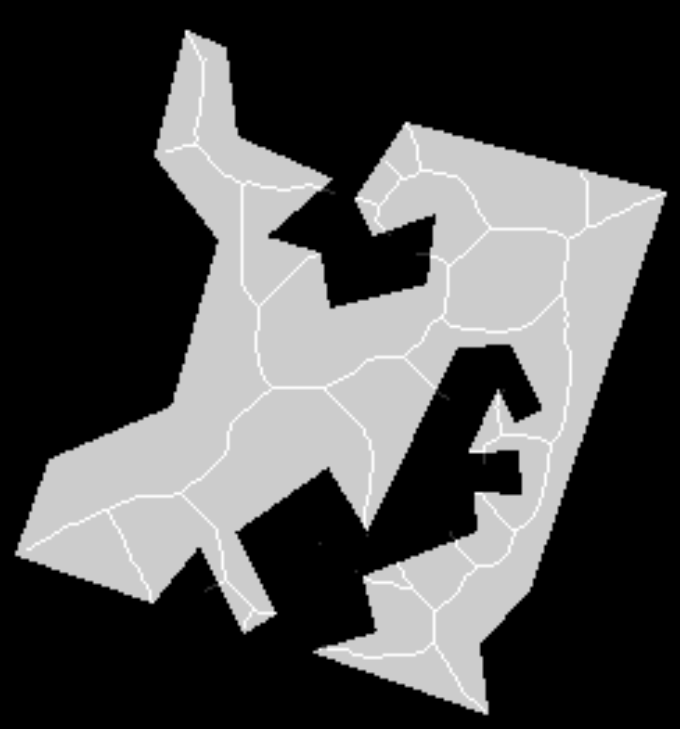
\includegraphics[width=0.7\linewidth]{latex/figures/Screenshot 2026-06-12 at 11.06.44.png}
    \caption[]{Morphological skeleton extracted from the free-space representation of the environment.}
    \label{fig-skeleton_free__}
    \end{figure}
    Once the waypoints are obtained, a graph is constructed and leaf nodes are extracted. In the graph, leaf nodes are defined by their single connection to the rest of the skeleton; these are treated as endpoints of the path.

    \begin{figure}[!htbp]
    \centering
    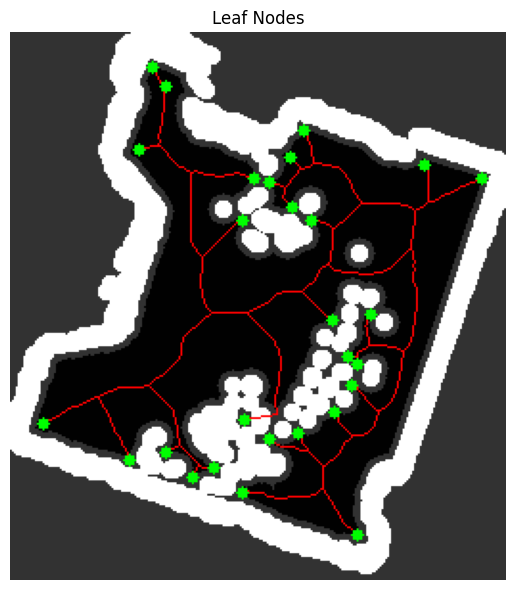
\includegraphics[width=0.99\linewidth]{content/figures/navigator_results/skeleton_tree_leaves.png}
    \caption{Leaf nodes identified on the skeleton graph, representing endpoints used during path generation.}
    \label{fig-skeleton_leaves__}
    \end{figure}
    
    Finally, starting from the leaf node closest to the robot, the full path is planned by recursively tracing the graph from the current leaf node to the nearest unvisited leaf node. This can be seen in Figure \ref{fig:full_path__}.

    \begin{figure}
        \centering
        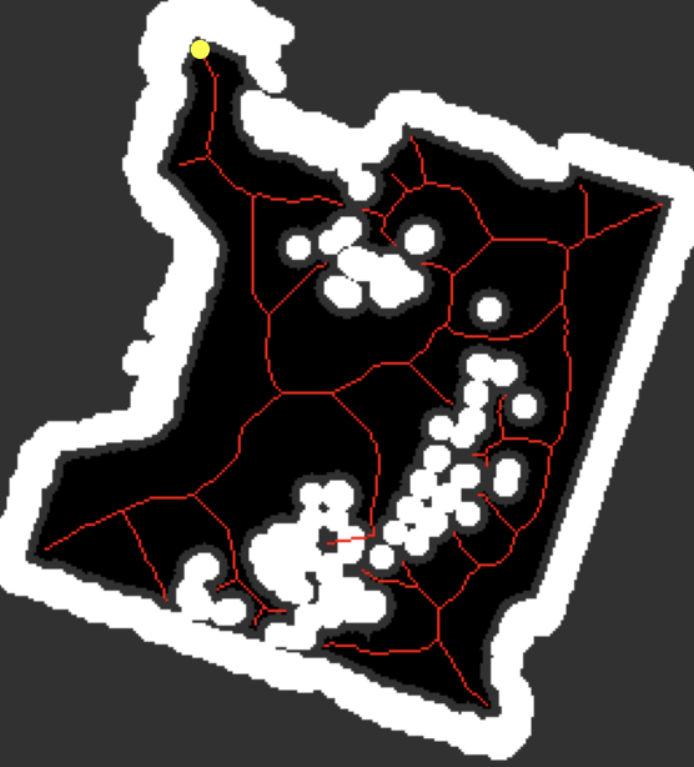
\includegraphics[width=0.7\linewidth]{latex/figures/Screenshot 2026-06-12 at 11.10.58.png}
        \caption{Fully planned path}
        \label{fig:full_path__}
    \end{figure}
    \paragraph{Grid-Based Spanning-Tree Planner}
    Secondly, a grid-based spanning-tree algorithm is used to plan a full coverage path over the map. This planner is based on the work of \cite{SpanningTree2001}.

    Unlike the skeleton planner, this planner uses the binary costmap directly. The binary costmap is further discretized to a grid whose resolution is a fraction of that of the original costmap, see Figure~\ref{fig-spanning_grid__}.

    \begin{figure}[!htbp]
    \centering
    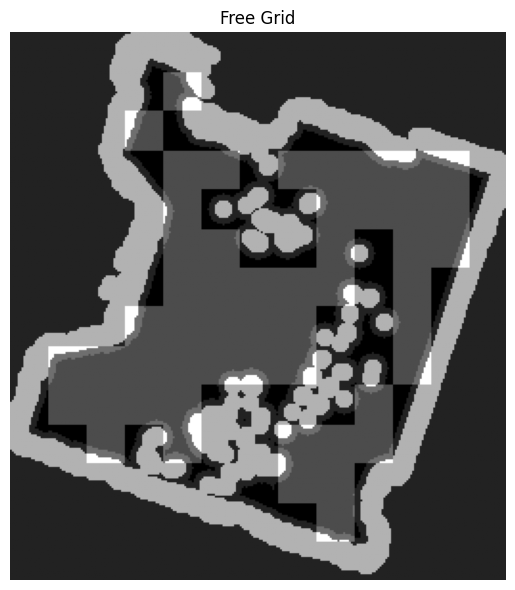
\includegraphics[width=0.7\linewidth]{content/figures/navigator_results/spanning_tree_grid.png}
    \caption[]{Downsampled free-space grid used to construct the spanning tree graph.}
    \label{fig-spanning_grid__}
    \end{figure}

    A depth-first search (DFS) is conducted over the free cells, from which sparse waypoints are created. This can be seen in Figure \ref{fig:fig-spanning_dfs__}.

    \begin{figure}
        \centering
        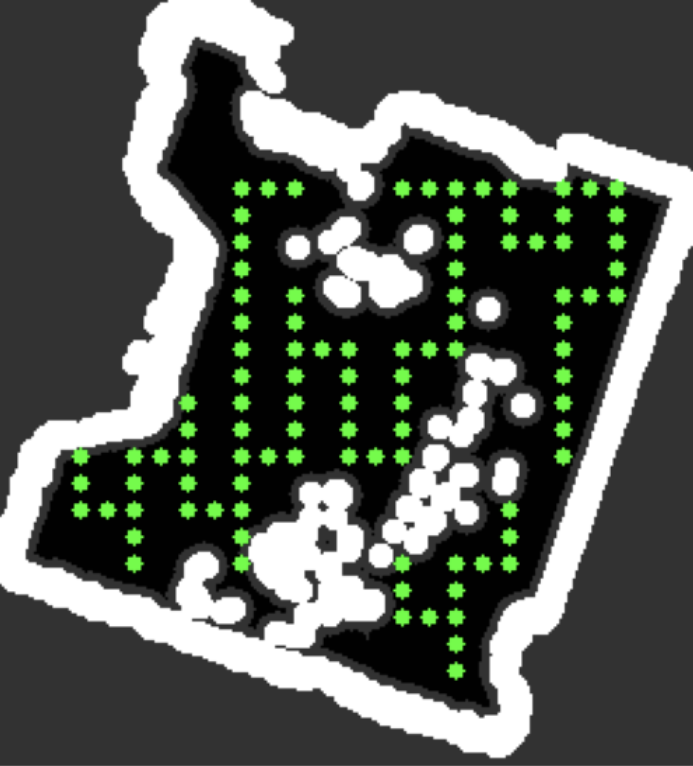
\includegraphics[width=0.7\linewidth]{latex/figures/Screenshot 2026-06-12 at 11.16.30.png}
        \caption{Depth-first search spanning tree generated over the free-space grid.}
        \label{fig:fig-spanning_dfs__}
    \end{figure}
    A black image with the same resolution as the original costmap is then created, and white squares with half the cell width are placed in the center of each cell and between adjacent cells. Waypoints are created from the contours of this tree. These waypoints represent a circumnavigation around the DFS tree.
    \begin{figure}[!htbp]
    \centering
    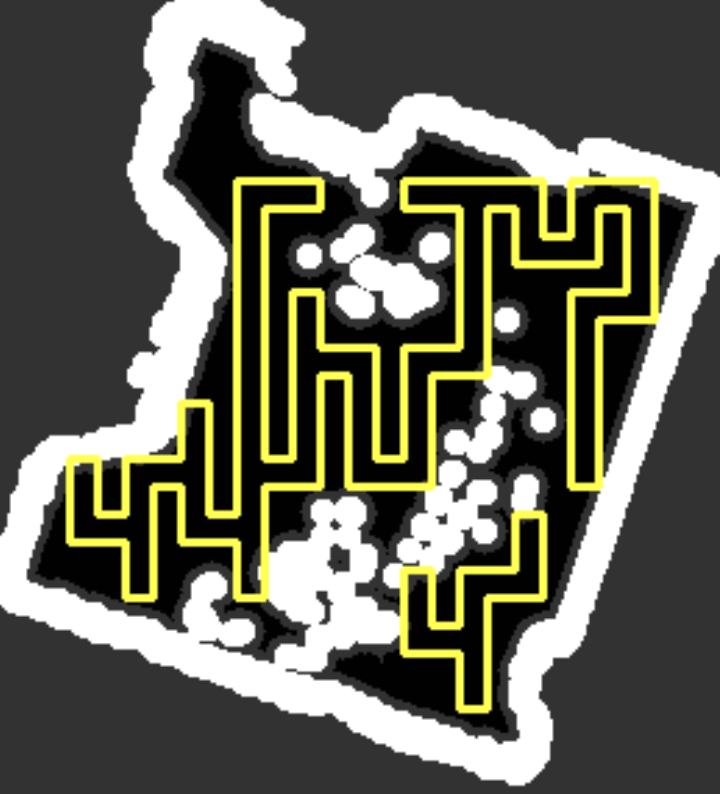
\includegraphics[width=0.7\linewidth]{latex/figures/Screenshot 2026-06-12 at 11.19.59.png}
    \caption[]{Coverage waypoints generated by tracing the contour around the spanning tree structure.}
    \label{fig-spanning_waypoints__}
    \end{figure}
    A segment from this circumnavigation is then removed from the path.

    \begin{figure}
        \centering
        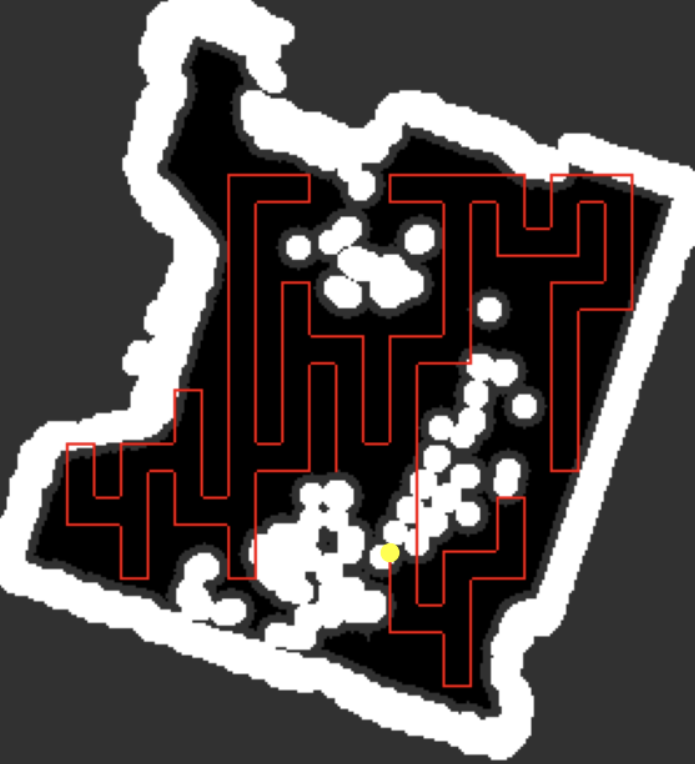
\includegraphics[width=0.7\linewidth]{latex/figures/Screenshot 2026-06-12 at 11.29.22.png}
        \caption{The path with circumnavigation removed.}
        \label{fig:placeholder}
    \end{figure}
    A lab cleanup robot must not blindly follow waypoints. If it does, it might collide with obstacles near the map boundary or collide with moving objects. \newline
    Nav2 implements several low-level real-time trajectory planners that plan inside the live-updating costmap \cite{macenski2023survey}. They handle how the waypoints are followed and how much influence the map ought to have on the generated trajectory. The system described in this section implements an MPPI controller \cite{williams2017mppi} due to its superior performance in highly dynamic environments \cite{elbouhy2024ros2planning}, such as labs where students or other people frequently walk. Other planners that were considered include DWB (Dynamic Window Approach Behavior-based) \cite{thrun1997dwa} and RPP (Regulated Pure Pursuit) \cite{macenski2023regulated}.
    \subsection{Robot Behavior}

    A common approach in robotics for navigation- and perception-heavy tasks is to use a global behavior tree that describes the robot's actions in different situations. This architecture, as shown in Figure~\ref{fig:tree}, is used here to describe and execute the cleaning strategy. The \textit{Py Trees for ROS} Python package is used to implement the behavior tree because of its thorough documentation and its native support in ROS 2.

    The behavior tree provides a hierarchical approach for coordinating navigation, perception, and cleaning actions. It also provides a clear structure for debugging. As seen in Figure~\ref{fig:tree}, the robot first explores the environment, then pauses its coverage task whenever an object is detected, approaches the object, checks whether it is still visible, picks it up, and places it in the appropriate bin. The complete tree is shown in Figure~\ref{fig:tree_full} in the Appendix, and the execution of the coverage task, including pausing and resuming, is described in Algorithm~\ref{alg:coverage_exec}.
    \begin{figure}[H]
        \centering
        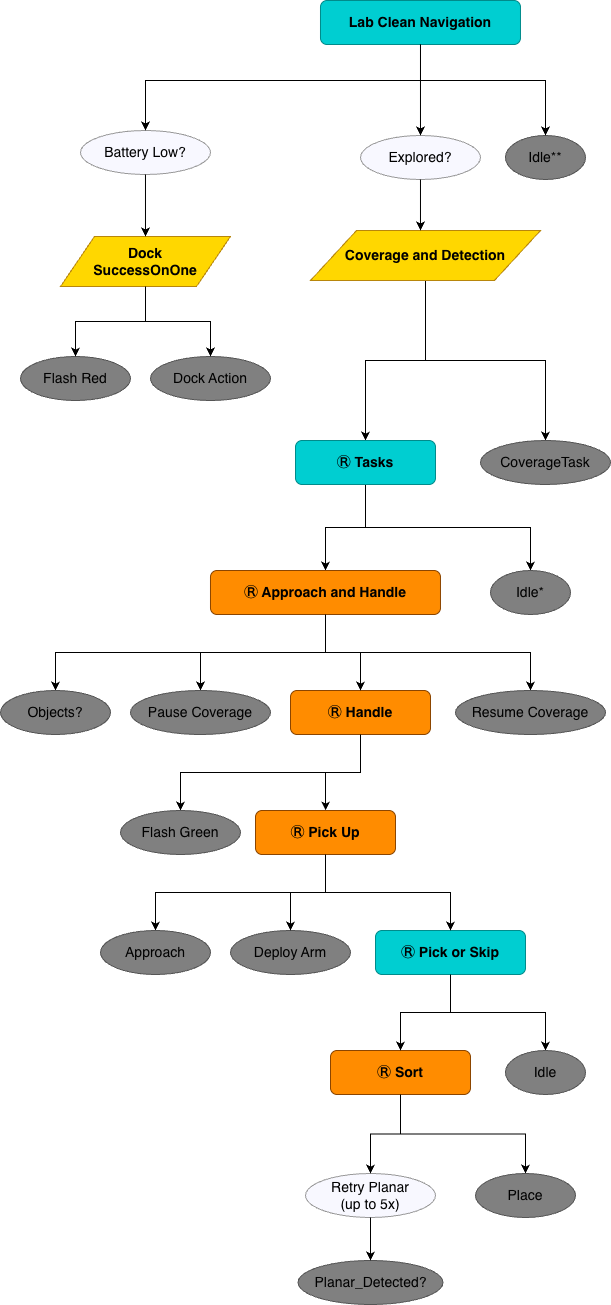
\includegraphics[width=0.78\linewidth]{latex/figures/labclean_tree.drawio-simple tree.drawio (1).png}
        \caption{Behavior tree (simplified)}
        \label{fig:tree}
    \end{figure}
    \subsection{Mechanical}

    The MIRTE Master platform provides a capable but general-purpose starting point for a laboratory cleaning robot. Out of the box, it offers omnidirectional mobility, a four-degree-of-freedom manipulator, and an integrated sensor suite. However, several of its design choices were not well-suited to the specific demands of autonomous waste collection and sorting. This section documents the physical modifications made to the platform: what was changed, why, and how each modification contributes to the overall system's ability to reliably detect, grasp, and sort laboratory objects.

    \subsubsection{Original MIRTE Master Platform}

    The original MIRTE Master hardware consists of three main parts:
    \begin{enumerate}
    \item \textbf{Mobile base}
    \item \textbf{Electronics}
    \item \textbf{Robotic arm}
    \end{enumerate}
    The mobile base utilizes four geared DC motors with Hall encoders, connected to 97 mm mecanum wheels. This configuration enables omnidirectional movement, which is useful for navigating in small indoor spaces. The base also contains rearward-facing ultrasonic sensors, an IMU, a 2D LiDAR and an RGBD (depth) camera.

    The electronics of the original platform are based on an Orange Pi 3B and a Raspberry Pi Pico H, following a two-tier software architecture that separates high-level task logic from low-level execution. The Orange Pi functions as the main computer, handling computationally intensive tasks. The Pico, as the embedded controller, handles lower-level control tasks such as driving the motors and reading lightweight sensor data. The MIRTE Master also includes a custom PCB to connect the motors, sensors, and power system in a structured manner, powered by a 5 Ah 12 V Li-ion Parkside drill battery. No significant changes were made to the electronics for this project.

    The robotic arm is mounted on top of the mobile base and has four degrees of freedom, which are driven by four serial bus servo motors of varying strengths. A gripper and RGBD camera are mounted at the end of the arm for object scanning and manipulation.

    The original hardware components can be seen in \href{https://matt-rbt.github.io/Lab-Cleanup-Robot-using-the-Mirte-Master-Platform/materials/}{Materials}.

    \subsubsection{Design Goals for the Modified Robot}

    Despite being a capable platform, several aspects of the original design presented practical limitations for this specific use case. The PMMA chassis plates proved brittle under load, cracking during early testing. The RGBD camera, mounted low at the front of the chassis, was too close to the ground to produce reliable depth estimates for small objects on the floor. The gripper's contact surfaces lacked the friction needed to reliably grasp small, smooth electronic components. Finally, the platform had no provision for storing or separating collected objects. These shortcomings directly motivated the modifications described in the following sections.

    The main design goals are:
    \begin{itemize}
    \item Increase the stiffness and reliability of the chassis.
    \item Add space for collecting and separating waste.
    \item Mount the camera in a position that enables object detection.
    \item Improve the battery mounting system.
    \item Improve cable management.
    \item Modify the gripper so it can pick up waste objects more reliably.
    \end{itemize}

    \subsubsection{Chassis Modifications}

    The original MIRTE Master chassis was designed as a general-purpose mobile manipulator base. For this use case, the robot also needed to carry waste bins.

    The chassis consists of six side panels and a top and a bottom plate. In the original model, the top and bottom plates were made of clear PMMA. Although PMMA allows the user to see the status of the electronics by looking at the LEDs on the inside, early testing of the MIRTE Master showed that it was not suitable, as attempts to assemble the robot often resulted in shattered plates. The fracture toughness of PMMA (0.7--1.1 MPa$\cdot$m$^{1/2}$), which is approximately 30 times lower than that of aluminium (23--35 MPa$\cdot$m$^{1/2}$), makes it prone to sudden brittle fracture under mechanical load. Therefore, the PMMA was replaced with aluminium. To still be able to see the status LEDs, the six side panels were 3D-printed using translucent PETG. Two separate waste bins were also added to the rear of the chassis, as they allow the robot to collect, store and separate objects after picking them up.
    \subsubsection{Gripper Modifications}

    The original MIRTE Master gripper is useful as a general robotic gripper, but the cleanup task requires it to reliably handle objects that vary widely in shape and size.

    The original gripper geometry is suitable for holding small and large objects; however, the gripping surface is not. Electronic components tend to have small areas of contact with the gripper, making slippage likely during lifting. To improve gripping performance, the contact patches are layered with soft 83A TPE, coated with an additional layer of Bison Rubber anti-slip coating.

    During the initial testing phase of the RGBD camera, it was found that the mounting point was too low for any objects close to the ground to be visible. Although the camera was originally intended to be mounted on the chassis, mounting it on the end of the arm proved beneficial for this project. In addition to the elevated vantage point, this allows for programmable viewing angles. Furthermore, the RGBD camera is now also used for object detection, making the secondary RGB camera unnecessary.

    \subsubsection{Current Design}
    The complete model can be explored using the interactive 3D interface on the \href{https://matt-rbt.github.io/Lab-Cleanup-Robot-using-the-Mirte-Master-Platform/mechanical/}{Mechanical} page of the online report. The CAD files can be found \href{https://cad.onshape.com/documents/ee158bec245e3fe46f63c9ce/w/a0c8c76ba94ff339073118d4/e/a16fbc4a88cf67fd9fba6368?renderMode=0&uiState=6a2aaef65092a9418fe6a8f1}{here}.

    \subsection{Manipulation}

    This section covers the articulation of the robotic arm that sits atop the MIRTE Master. Since there is hardly any competition in this space, the market leader, MoveIt 2, was used to move the arm. MoveIt 2 provides a well-documented API and directs the vast majority of computations regarding (inverse) kinematics of robotic arms and the trajectory planning thereafter \cite{moveit2_api}.

    The package is already installed on the MIRTE Master and has previously been used, with limited success, to move MIRTE's arm \cite{mirte_moveit_tutorial}. However, this implementation resulted in the end effector (the tip of the arm; the wrist) being positioned more than 10 cm off-target. For a machine needing to pick up objects smaller than 6 cm, this is unacceptable. Therefore, an improved version is required. To this end, the designed behavior contains a number of improvements and concessions:

    \subsubsection{Changes}
    \begin{itemize}
    \item The previously missing configuration file, \texttt{moveit\_cpp.yaml}, which contains additional parameters (specifically for OMPL, the motion planner), was created and added.

    \item To accommodate the fact that MIRTE's arm can only move with four degrees of freedom (DOF) instead of the six assumed by MoveIt 2, planning is performed strictly for position, ignoring any orientation component of a goal pose entirely. Together with the first point, this made it possible to use more precise methods from the Move Group Interface to plan and execute movements instead of \texttt{setApproximateJointValues()}. The resulting positional accuracy is in the order of millimetres, although alignment of the gripper must be configured separately.

    \item Functionality has been added to ensure that the gripper points the depth camera downward at an angle relative to the ground, so that the camera can correctly detect the floor itself and any objects on it. When an object is detected and needs to be classified, the robot points the depth camera straight down relative to the world axes for classification. This ensures that any approached object is directly below the camera. As a result, the gripper camera has a constant and uniform background, increasing classification confidence levels.

    \item An action server has been developed that provides feedback to a potential action client. The server can receive goals in several formats:
    \begin{itemize}
    \item By specifying the name of a joint state predefined in the robot's description files.
    \item By supplying a goal pose relative to MIRTE's frame \texttt{base\_link}.
    \end{itemize}
    The action server moves the arm in a way that satisfies the goal, if possible. The wrist joint can be moved separately to allow fine adjustment of the gripper's orientation. Similarly, the gripper can be controlled either by specifying a named state or by directly assigning a desired clamping angle. The gripper will move accordingly, if possible.
    \end{itemize}

    Together, these modifications facilitate the movement of the robotic arm for this specific project and enable the creation of additional custom manipulation modules for future projects.
    \subsection{Perception}
    Perception is responsible for object detection, classification, and spatial localization. In this study, two object-detection and localization approaches were evaluated: a \textbf{2D detection and depth-projection} approach and a 3D segmentation approach based on \textbf{point-cloud clustering}. For classification, a classical computer-vision approach and a model-based approach were both considered.

    Initially, the goal was to distinguish between graspable and non-graspable objects and between electronics and non-electronics. However, because the standard MIRTE Master platform had limited camera quality and limited computational resources, the final scope was reduced to two practical classes: graspable versus non-graspable and colourful versus greyscale. This choice was made to keep the system feasible within the available hardware and to focus the evaluation on the most relevant objects for the laboratory-cleaning task.

    A custom YOLO-based detector was trained on a small labelled dataset collected from the onboard camera, while the 3D pipeline used point-cloud filtering, plane removal, and clustering to estimate the position and orientation of candidate objects. The combination of these two perception streams was then used to support the grasping and sorting process.
    \subsubsection{Perception 2D}
    For determining the type, and possibly the distance of objects, a YOLO26 (`You Only Look Once-26') object-detection model was used. A dataset was created by recording videos using the USB camera included in the MIRTE Master hardware package, from which one in every fifteen frames was extracted for the training dataset. A figure of four frames in different environments is shown below in Figure \ref{fig_trainingdataset}.
    \begin{figure}[!htbp]
    \centering
    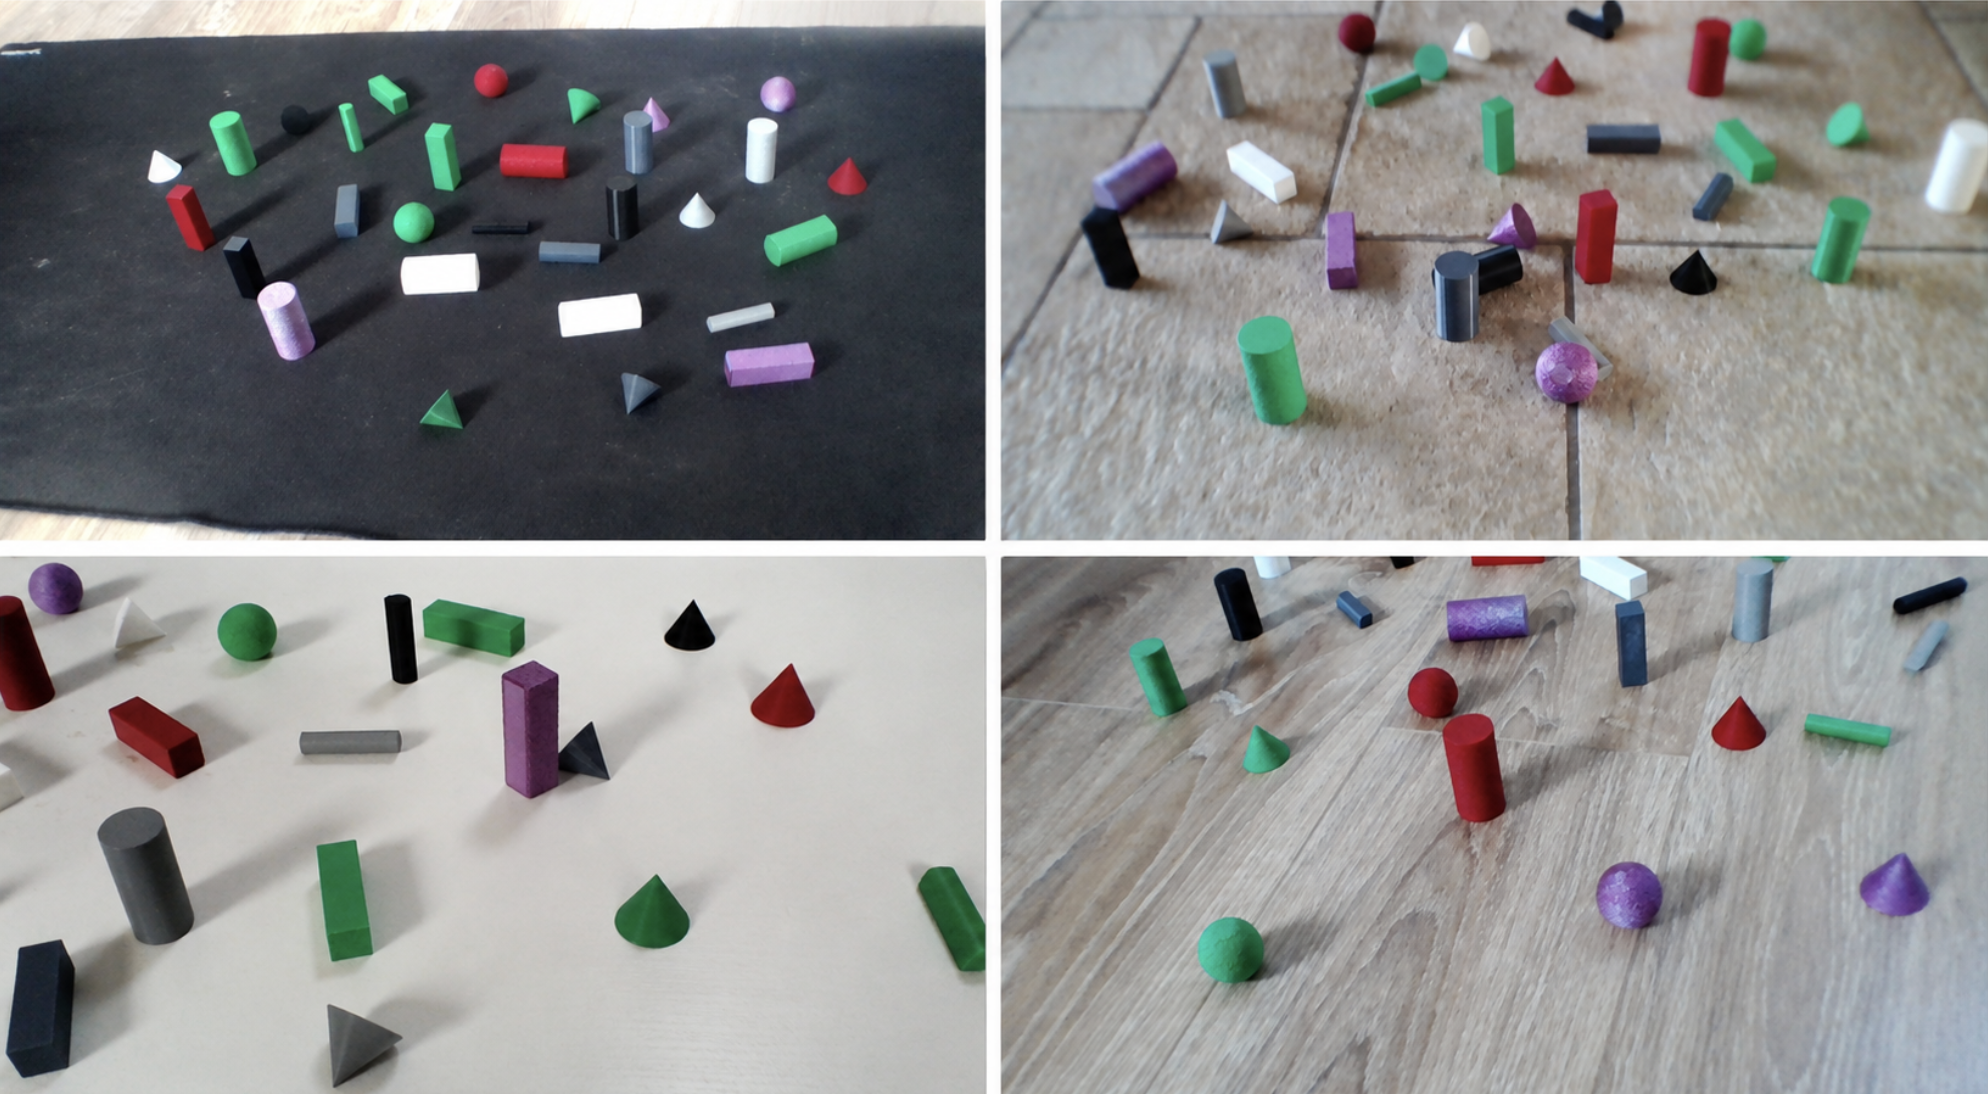
\includegraphics[width=0.99\linewidth]{latex/figures/Screenshot 2026-06-11 at 11.59.18.png}
    \caption[]{Picture of four individual frames}
    \label{fig_trainingdataset}
    \end{figure}
    
    \paragraph{Why YOLO26 Was Used}
    The YOLO object-detection family is well established, with YOLO26 \\
    \cite{ultralytics_yolo26} being the most recent generation. YOLO26 was chosen because the robot has to detect and classify objects from a live camera on the MIRTE Master platform, which has limited processing power because it uses an Orange Pi 3B. Object detection with limited processing power requires a lightweight model with fast inference times while still maintaining accuracy. YOLO26 is suitable for this because it was designed with deployment on low-power devices in mind. It uses NMS-free inference in its post-processing pipeline, simplifies bounding-box predictions, and supports deployment formats commonly used for low-power devices \cite{yolo26keyarchitecturalenhancements}.
    
    In this case, the RK3566 NPU of the Orange Pi 3B can be used to improve performance by reducing the total inference time \cite{Yolo11RK3566}. For this model, the Nano variant of YOLO26 was chosen to minimize inference times. Another benefit of YOLO26 over the older variants is its support for oriented bounding boxes. Unlike standard bounding boxes, oriented bounding boxes also estimate the rotation of recognized objects \cite{2026ultralyticsyoloevolutionoverview}. This could be useful for complex grasping tasks where the orientation of the gripper is crucial. However, this project only uses standard object detection.
    \paragraph{Training}
    The training data was annotated manually using Label Studio. Initially, roughly 280 frames were captured in four different environments. Due to a large amount of blurring within the images, about 100 pictures were deleted. Of the remaining 180 pictures, 60 were imported into Label Studio and labelled per colour: green, red, purple, white, light-grey, dark-grey and black. In total, 1206 bounding boxes were drawn. A test of the perception model performed during training is shown in the figure below.

    \begin{figure}[!htbp]
    \centering
    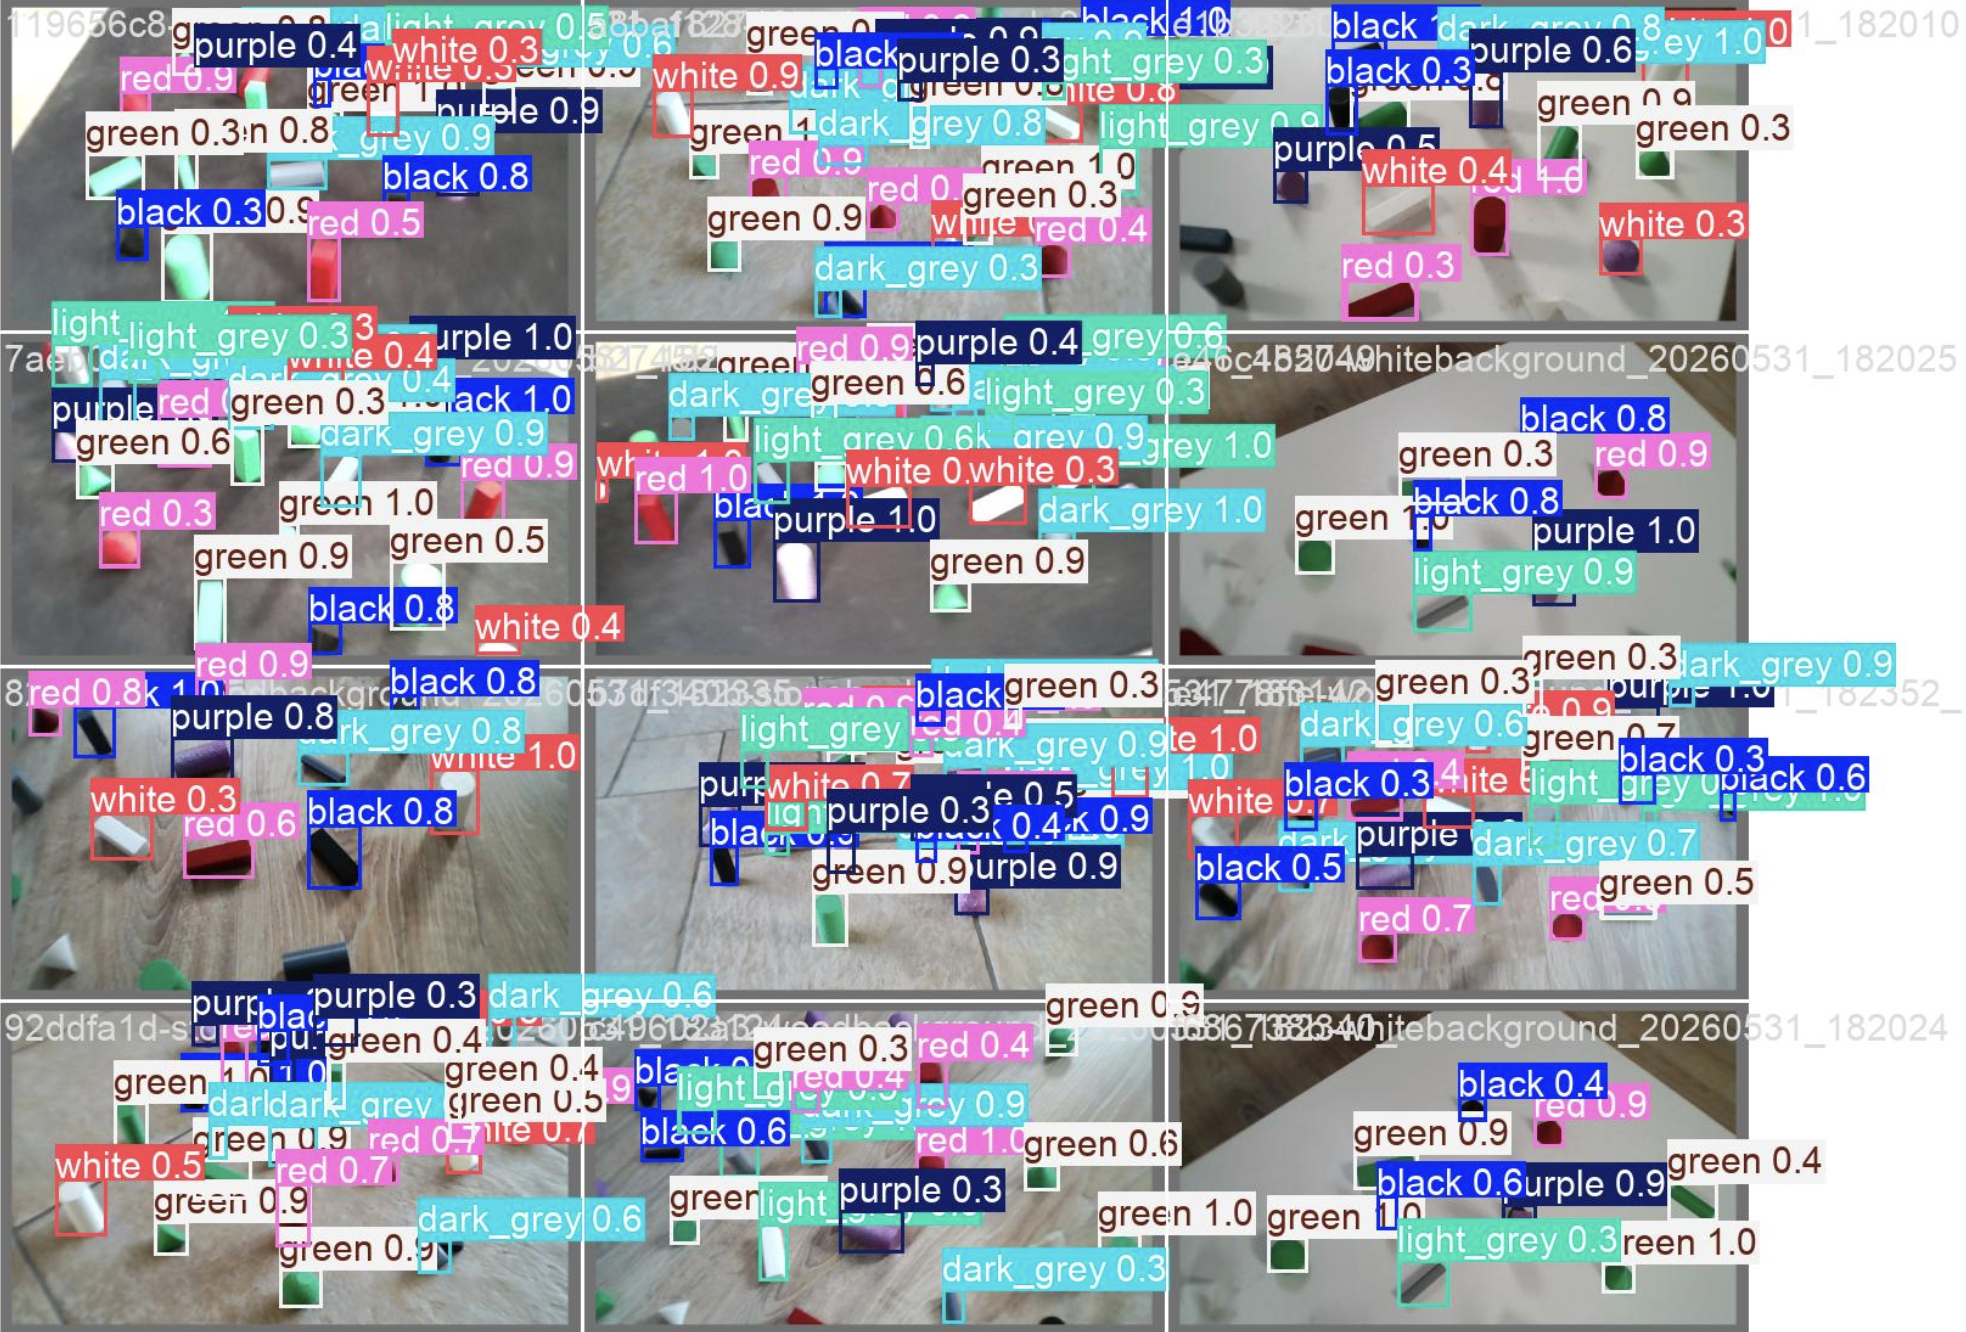
\includegraphics[width=0.99\linewidth]{latex/figures/Screenshot 2026-06-11 at 12.01.41.png}
    \caption[]{The tests performed during training.}
    \label{fig_trainingdatasetresults}
    \end{figure}
    %\smallskip
    The curves in the figure below show that the model converged during training. This means that the model actually learns while training instead of making random or unstable decisions.
    
    \begin{figure}[!htbp]
    \centering
    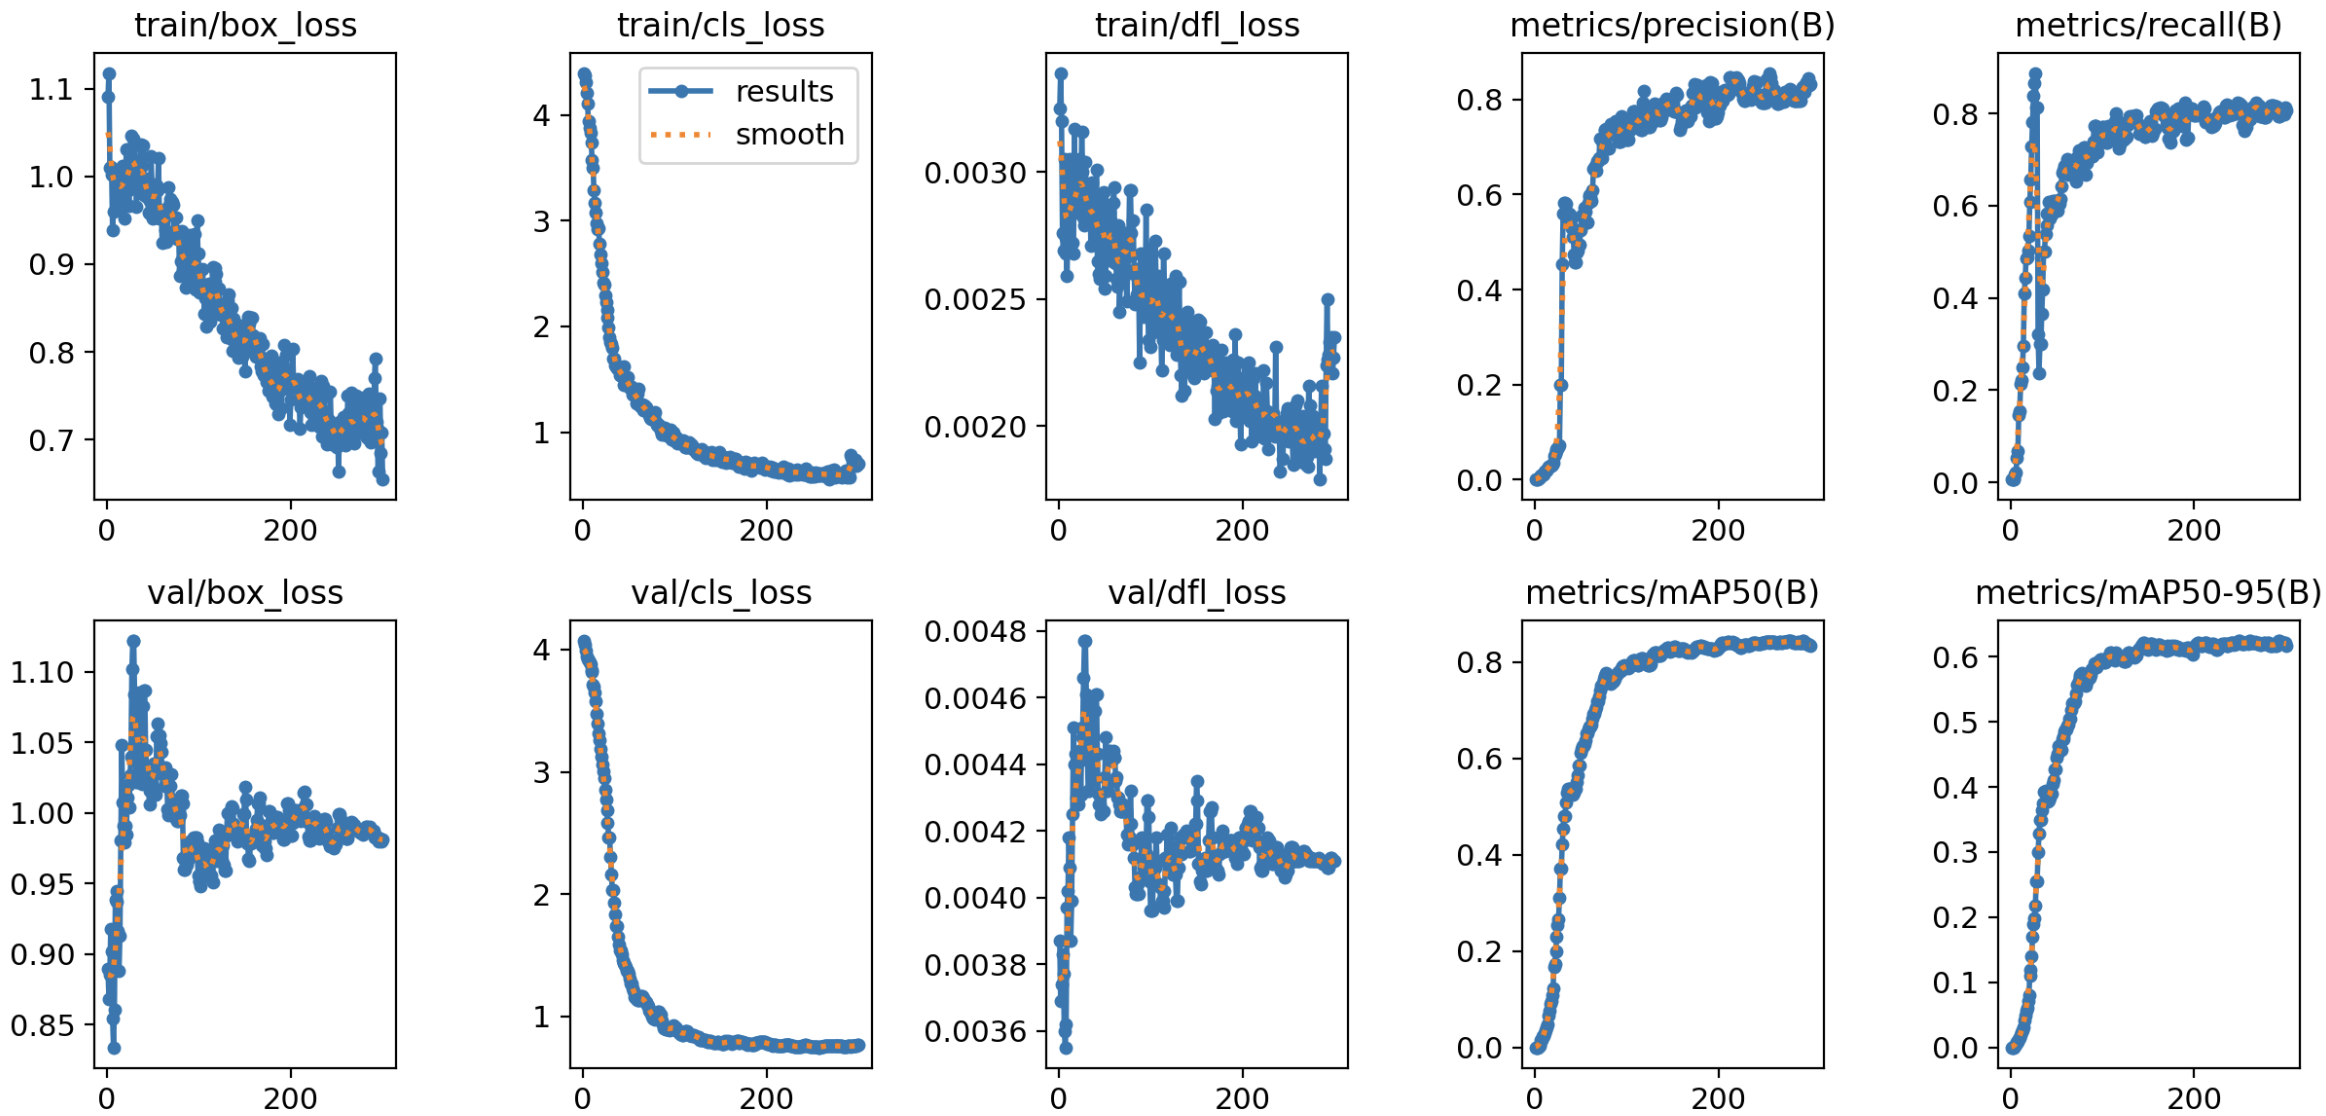
\includegraphics[width=0.99\linewidth]{latex/figures/Screenshot 2026-06-11 at 12.03.07.png}
    \caption[]{Plots of training results per epoch}
    \label{fig_trainingdatasetplots}
    \end{figure}

    The normalized confusion matrix shows how well classes are recognized by the model. As shown in the figure below, most classes are classified correctly, as indicated by the strong diagonal values. However, light-grey objects were among the least correctly identified objects, because changes in exposure and lighting often caused the model to classify them as background. Some objects were missed (classified as background), a small number of objects were misclassified, and some objects, such as dark-grey and white ones, were confused with light-grey.
    \begin{figure}[!htbp]
    \centering
    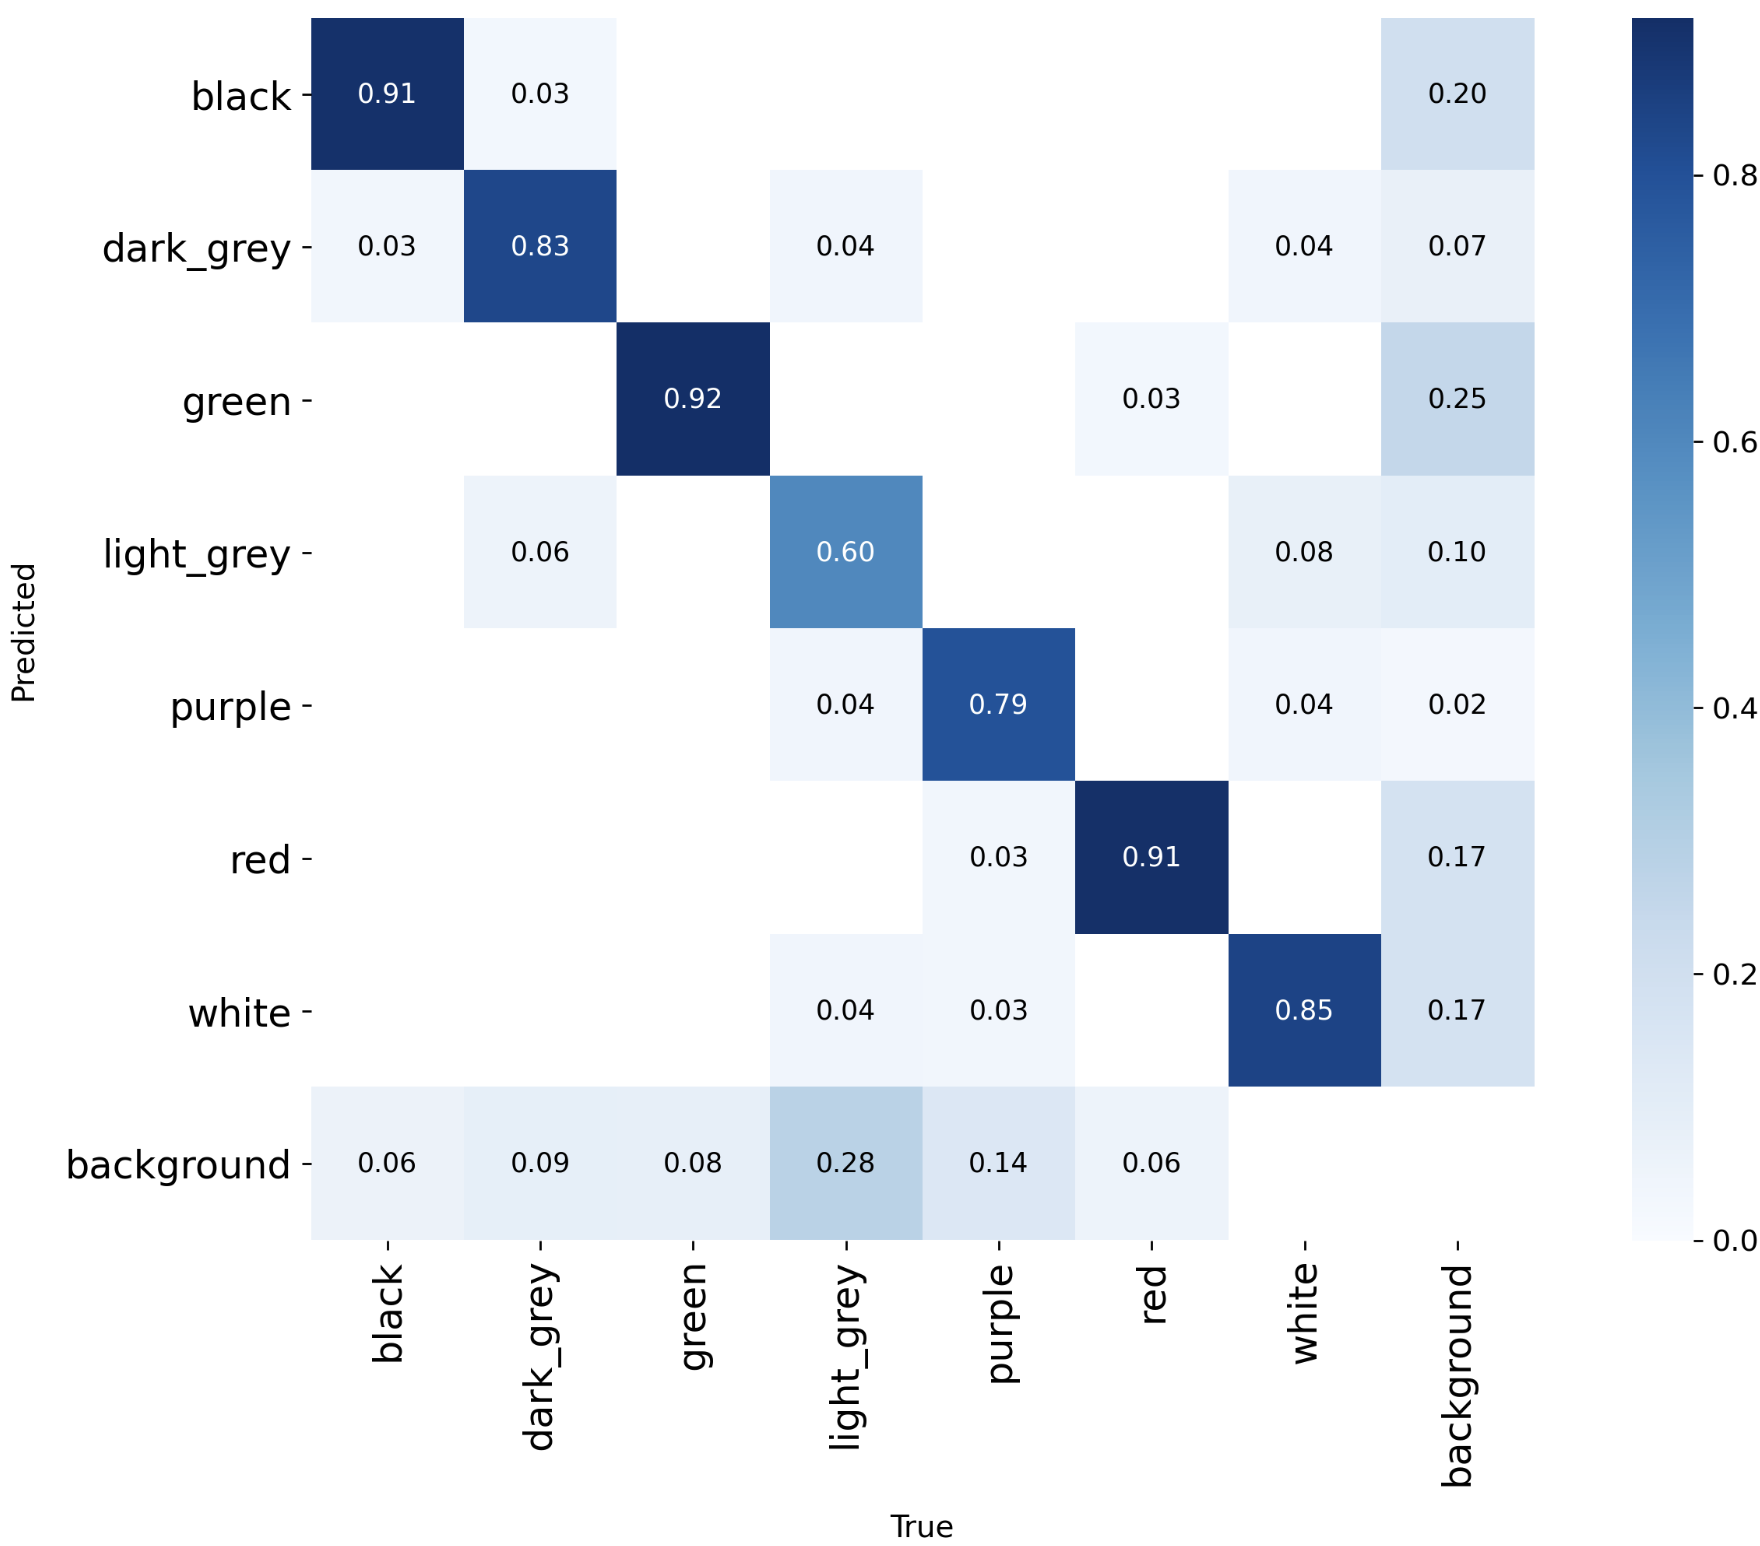
\includegraphics[width=1.01\linewidth]{latex/figures/Screenshot 2026-06-11 at 12.03.55.png}
    \caption[]{Normalised confusion matrix}
    \label{fig_confusionmatrix}
    \end{figure}
    A figure of the F1 confidence curve is shown below. This curve shows how the F1 metric, which combines precision (how many objects were correctly predicted) and recall (how many objects were correctly found), changes with the confidence threshold of the model. The curve shows that a good starting confidence threshold would be 0.3--0.35.
    \begin{figure}[!htbp]
    \centering
    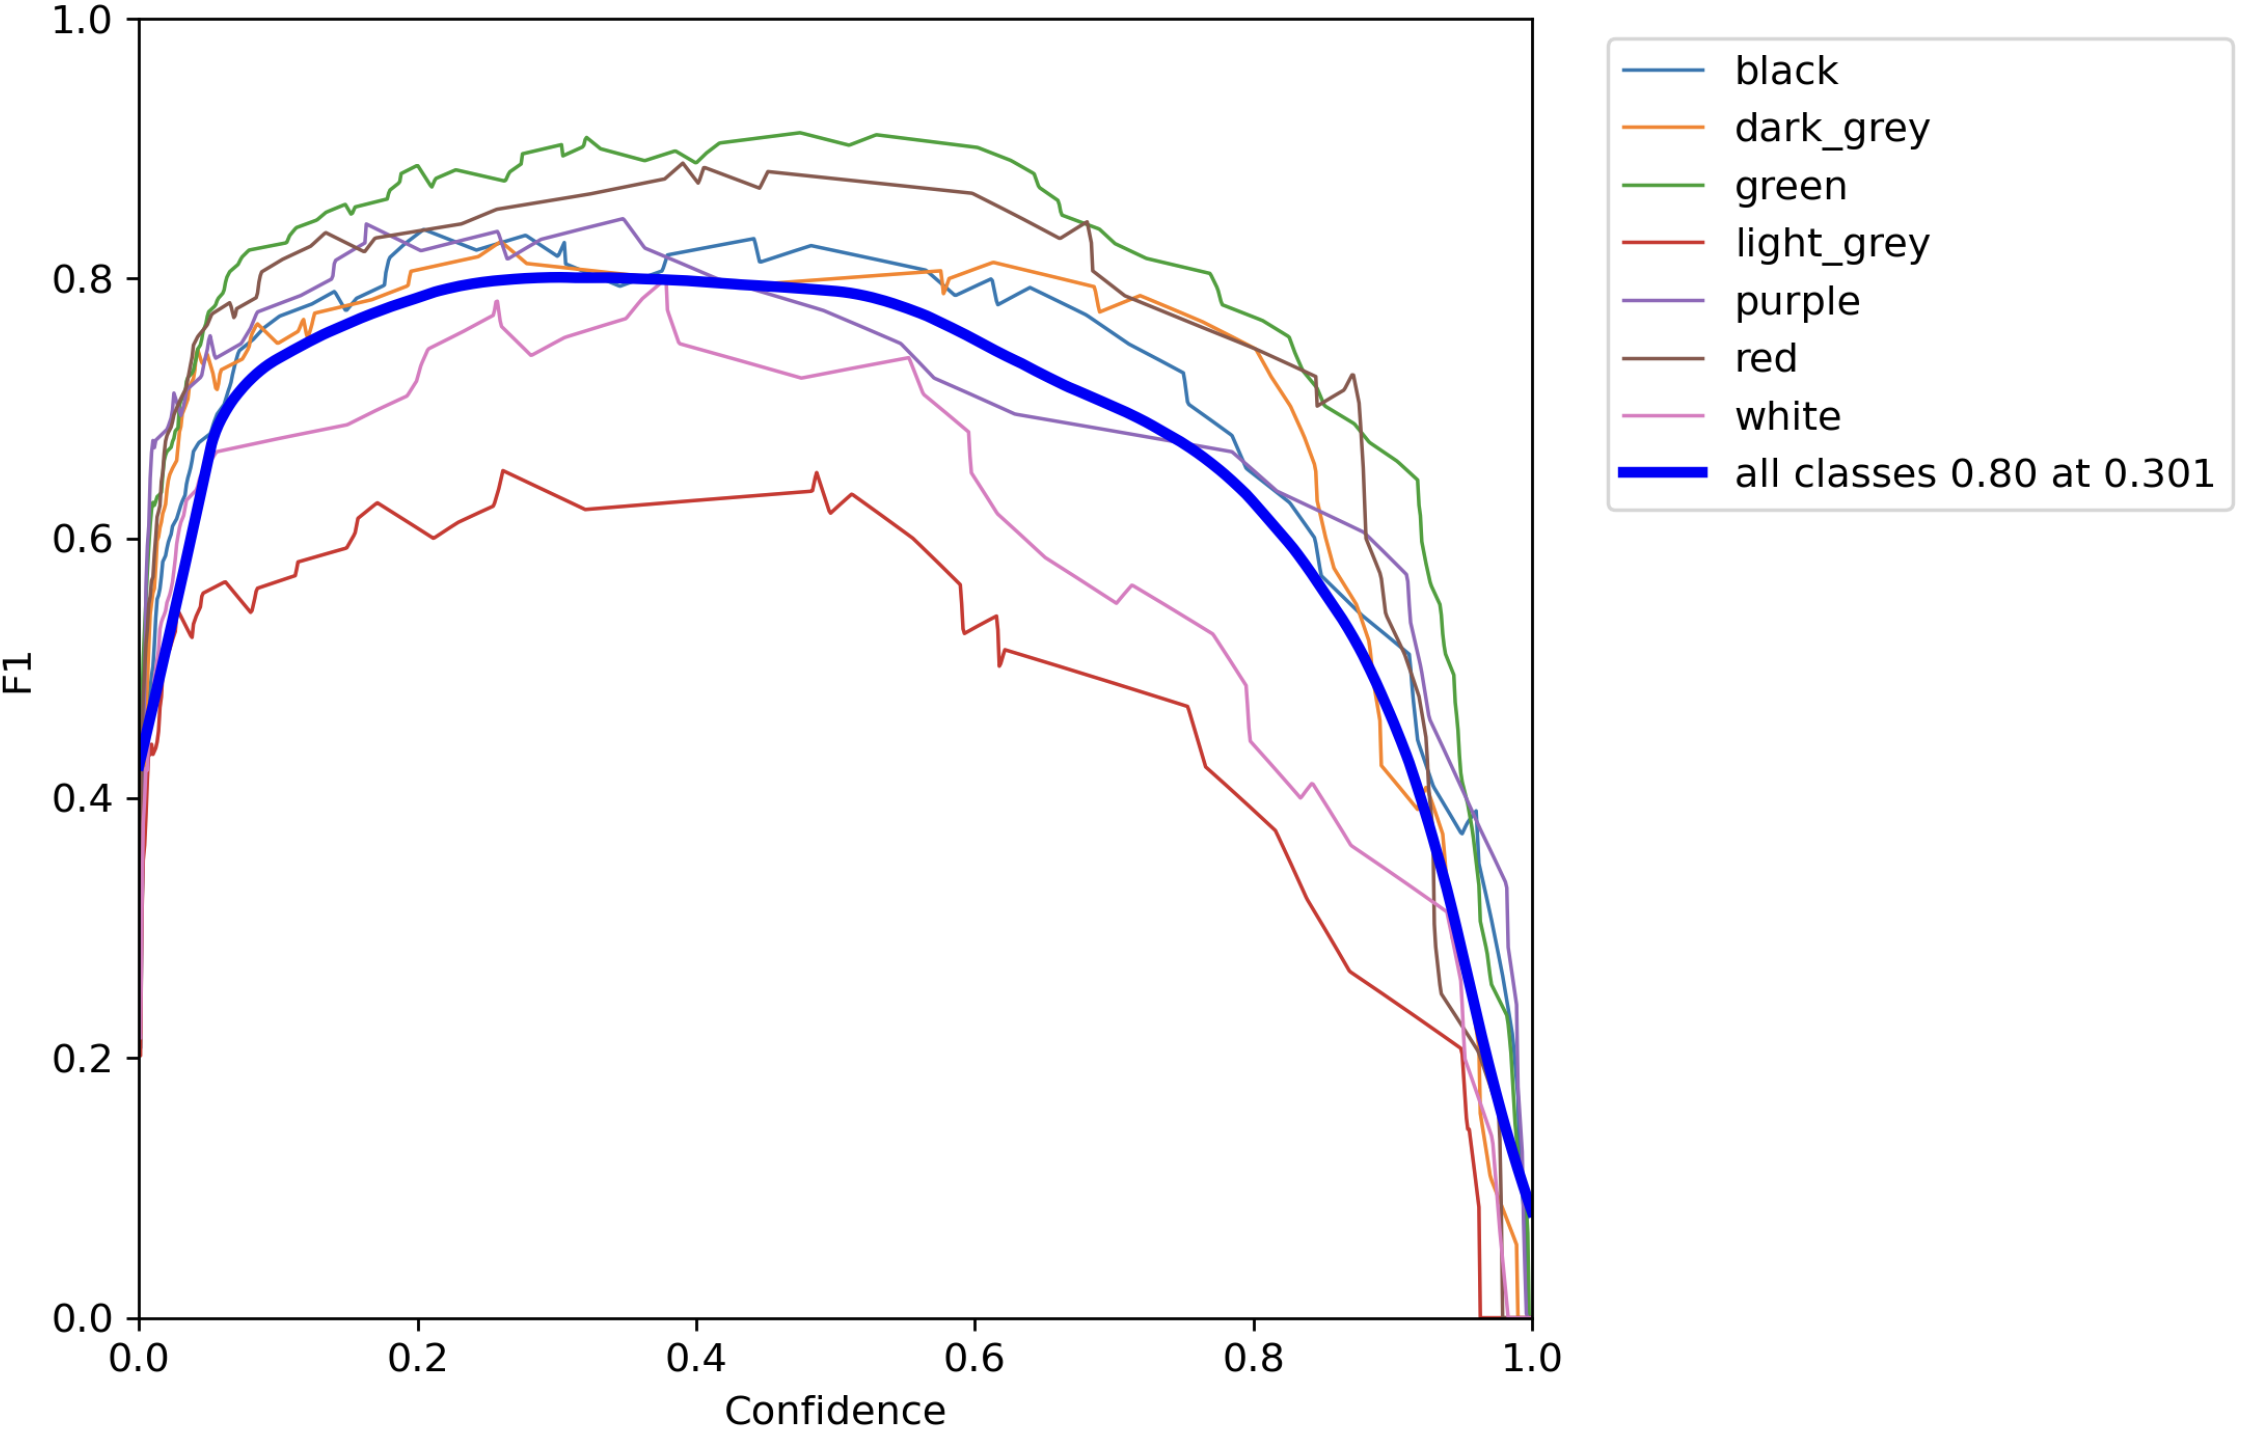
\includegraphics[width=1.02\linewidth]{latex/figures/Screenshot 2026-06-11 at 12.05.07.png}
    \caption[]{BoxF1 curve}
    \label{fig_boxf1curve}
    \end{figure}
    
    \subsubsection{Perception 3D}
    \paragraph{Point Cloud-Based Object Localization}

    To determine the exact location of graspable objects around the MIRTE Master, the data gathered and transmitted by the camera must be interpreted. One effective method for achieving this is through the use of point clouds.
    
    As the name suggests, point clouds are collections of points that represent a three-dimensional space. These points may contain a variety of information, but the most important characteristic of a point during this project is its position, represented by its \textit{x}, \textit{y}, and \textit{z} coordinates. During this project, the \texttt{Open3D} library was used to process the point cloud. This particular library has been selected because of its user-friendly API and popularity over PCL \cite{zhou2018open3d}.
    
    Planes are detected using the Random Sample Consensus (RANSAC) algorithm. This algorithm picks a number of points from the point cloud at random and fits a plane through them. It then evaluates which points in the point cloud are within the given distance from the plane \cite{Randomsampleconsensus}. With this method, point clouds can easily and quickly be filtered such that only the important parts, namely the clusters of points representing small objects on the ground, remain.
    
    Next, a clustering algorithm called DBSCAN (Density-Based Spatial Clustering of Applications with Noise) is used. The algorithm evaluates the remaining points in the point cloud and determines the cluster to which they belong \cite{DBSCAN}. Afterwards, the identified clusters can be converted into bounding boxes, determining an object's position and orientation, as well as its dimensions.
    Below, Figure~\ref{og_pc__} and Figure~\ref{bounding_boxes__} show the input and output of the point cloud pipeline.
    
     \begin{figure}[!htbp]
     \centering
     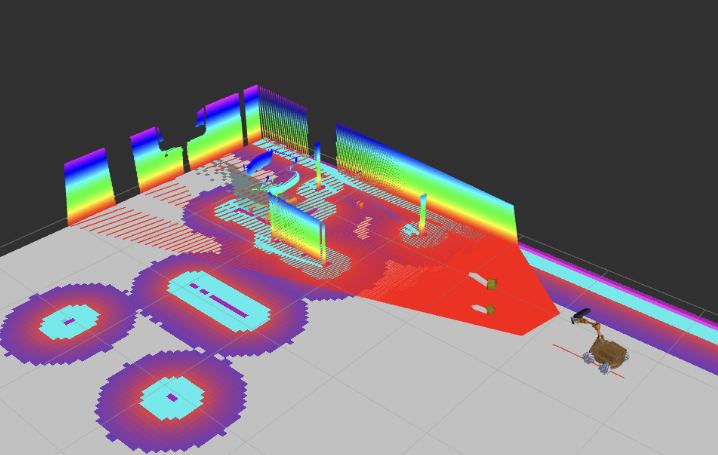
\includegraphics[width=0.99\linewidth]{latex/figures/Screenshot 2026-06-12 at 10.46.43.png}
     \caption[]{The point cloud as received from the camera topic}
     \label{og_pc__}
     \end{figure}
    
     \begin{figure}[!htbp]
     \centering
     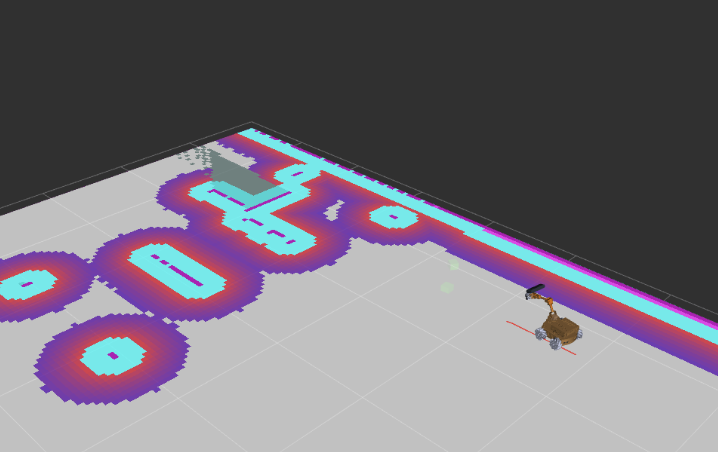
\includegraphics[width=0.99\linewidth]{latex/figures/Screenshot 2026-06-12 at 10.47.43.png}
     \caption[]{The resulting bounding boxes}
     \label{bounding_boxes__}
     \end{figure}
    
     Any objects that are part of the costmap are excluded, leaving only these bounding boxes.
    \subsubsection{Complete Point Cloud Processing Pipeline}
    This section shows the practices employed to process the point cloud received from the camera topic \texttt{/camera/depth/points}. Even though the inner workings of the specific functions used are outside the scope of this project, their influence is highlighted here to show their importance.

    For completeness, a point cloud is included below to give an impression of what the input of the pipeline looks like as received from the point cloud topic.

    To do this, a sample point cloud has been saved from the Gazebo simulation and is used as the input to a filtering pipeline built with the Open3D Python library:
    \begin{itemize}
    \item steps:
    \begin{itemize}
    \item Crop the point cloud to include only points below a given height.
    \item Copy a downsampled version of the point cloud to speed up future calculations.
    \item Iteratively detect planes and remove the corresponding points from both point clouds. From there, the downsampled point cloud will not be used anymore.
    \item Detect clusters from the remaining points.
    \item Create bounding boxes for these clusters.
    \item Reject boxes that overlap with the costmap.
    \end{itemize}
    \end{itemize}

    Any remaining bounding boxes are published as detected objects.

    The entire pipeline, including the individual effect of each step, is shown below:

    First, the original point cloud is created from the camera's depth image, as shown in Figure~\ref{pcp_og}.

    \begin{figure}[!htbp]
    \centering
    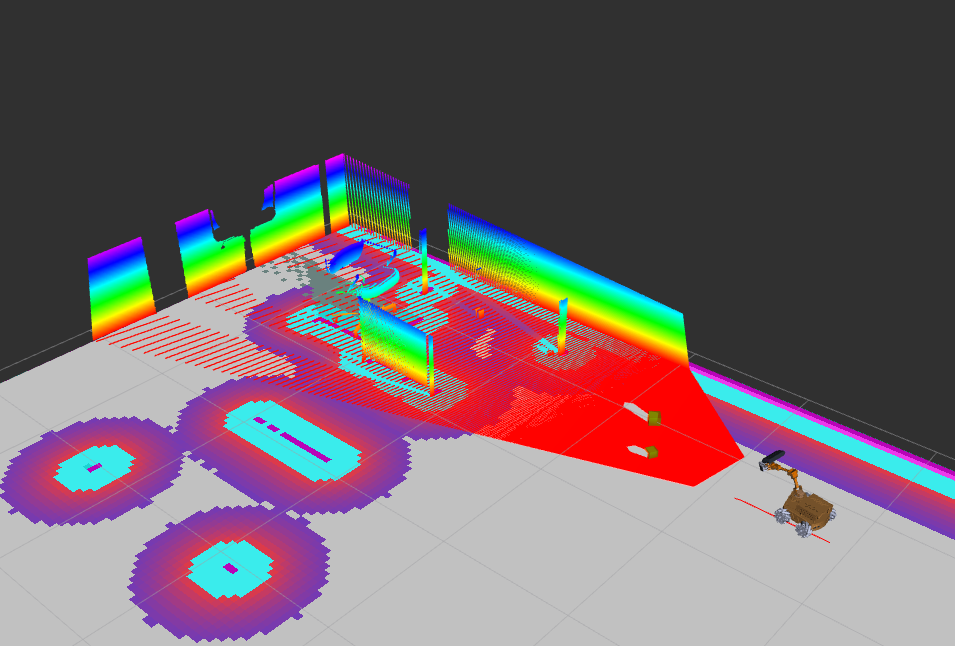
\includegraphics[width=0.9\linewidth]{content/figures/og_pc.png}
    \caption[]{The point cloud as received from the camera topic including the eventual bounding boxes}
    \label{pcp_og}
    \end{figure}

    Next, this point cloud is downsampled. Note that the resolution afterwards is still quite high. This is because the objects are very small, and reducing the resolution dramatically would lose details of these objects, reducing bounding-box accuracy. An example is shown below in Figure~\ref{pcp_downsampled}.

    \begin{figure}[!htbp]
    \centering
    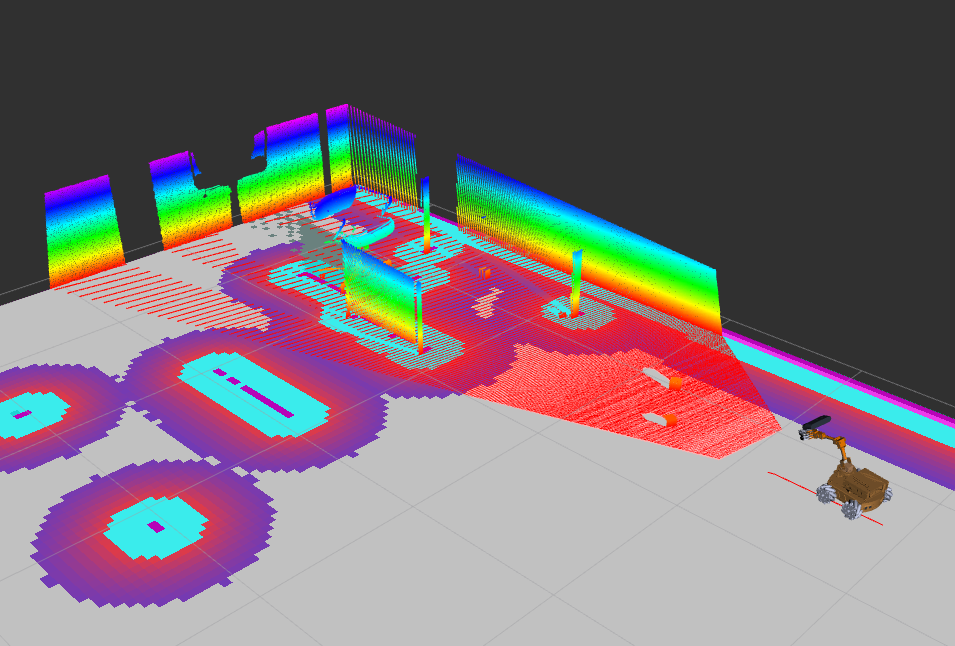
\includegraphics[width=0.9\linewidth]{content/figures/downsampled.png}
    \caption[]{The downsampled point cloud}
    \label{pcp_downsampled}
    \end{figure}

    In the downsampled point cloud, planes are detected using RANSAC plane segmentation \cite{Randomsampleconsensus}. With this, large planes such as walls and tabletops are discarded from the point cloud, as can be seen in Figure~\ref{pcp_segmented}.

    \begin{figure}[!htbp]
    \centering
    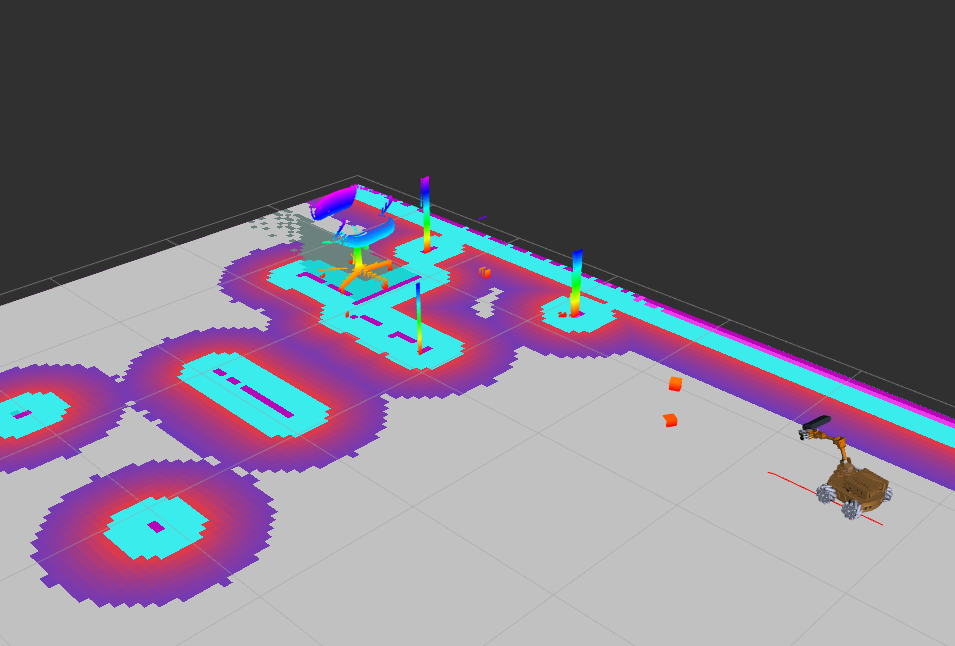
\includegraphics[width=0.9\linewidth]{content/figures/planeSegmented.png}
    \caption[]{The plane-segmented point cloud}
    \label{pcp_segmented}
    \end{figure}
    Now, the remaining points are cross-referenced with the costmap obtained during mapping. Any point that lies on the costmap is excluded from the point cloud, resulting in the point cloud depicted in Figure~\ref{pcp_exclusive}.

    \begin{figure}[!htbp]
    \centering
    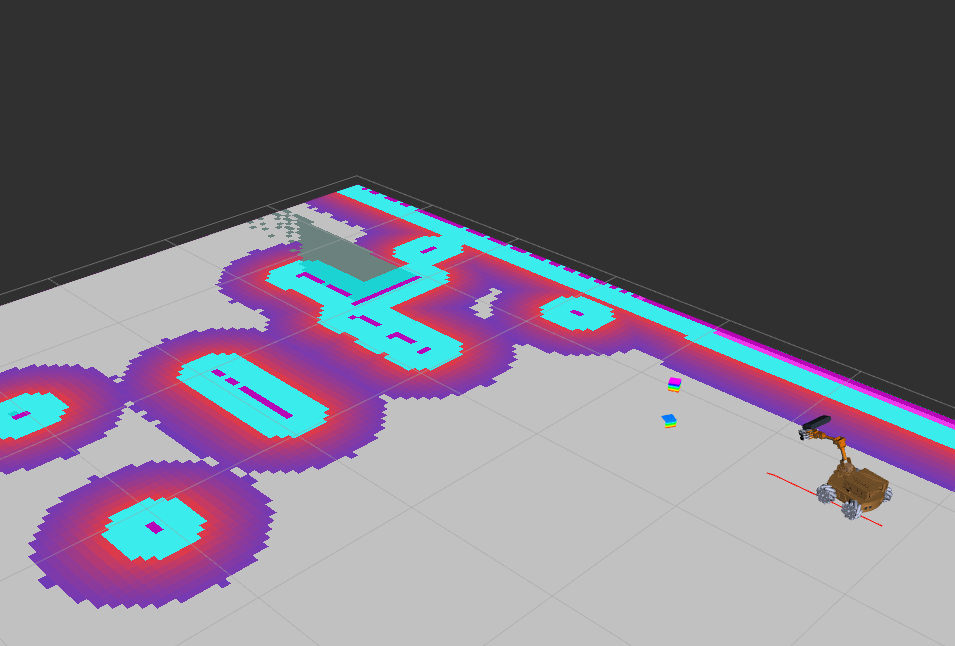
\includegraphics[width=0.9\linewidth]{content/figures/ExclusivePointCloud.png}
    \caption[]{The point cloud containing only points belonging to free objects}
    \label{pcp_exclusive}
    \end{figure}

    Finally, the remaining points are converted to clusters using DBSCAN \cite{DBSCAN}. This enables the construction of a bounding box for each cluster, each of which represents an object. Bounding boxes, however faint, can be made out in Figure~\ref{pcp_boxes} below.

    \begin{figure}[!htbp]
    \centering
    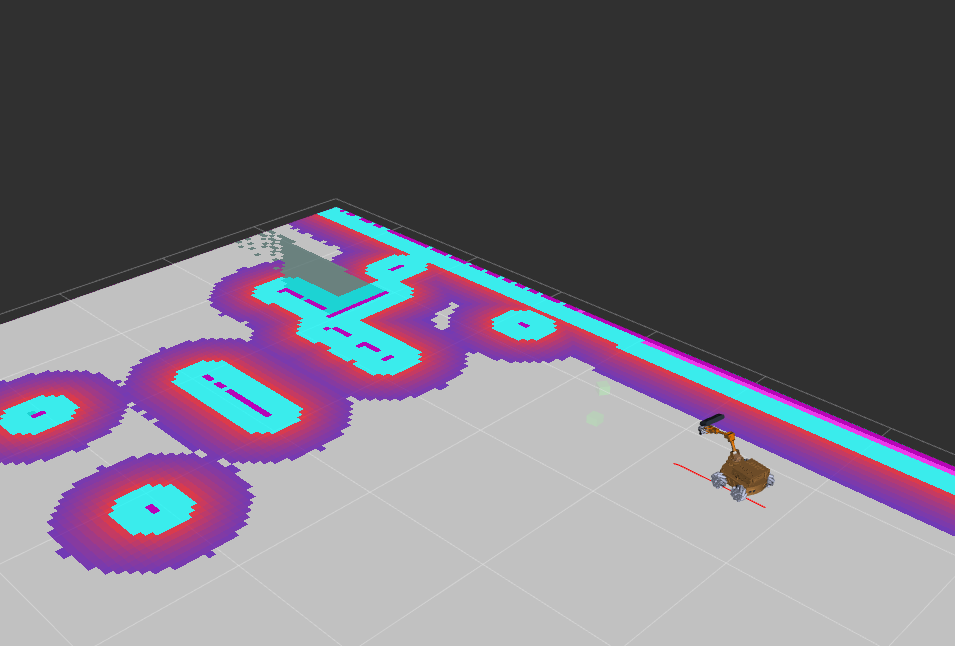
\includegraphics[width=0.9\linewidth]{content/figures/boundingBoxes.png}
    \caption[]{Bounding boxes (in front of the robot) are drawn around the remaining clusters.}
    \label{pcp_boxes}
    \end{figure}

    Information about these bounding boxes is then published on a ROS 2 topic, which is later used to approach and pick up the corresponding objects.

\section{Implementation}
\begin{paracol}
    {2}

    This section describes the transition from simulation-based development to real-world testing on the MIRTE Master platform and the practical requirements involved in doing so.

    To compare the implemented approaches, the study focused on practical performance indicators: whether the robot could complete a coverage run without losing track of its pose, whether objects could be detected and localized reliably, and whether manipulation could be executed accurately enough to place objects in the correct bin. These measures were used to evaluate the different planners and perception components.

    The programs required for lab cleanup operation are started from two launch files; the first launches the navigation, perception and manipulation stacks, while the second runs the behavior tree. This setup allows different behavior trees to be tested without restarting the other subsystems. A brief description of each subsystem's implementation is given below.

    \paragraph{Coverage Navigation}
    The coverage navigation system is implemented as an action server, meaning it plans and executes the coverage path in response to a request from an external client. The request specifies which coverage planner to use. As described in Section~\ref{sec:coverage}, the coverage task is executed as a sequence of waypoint segments. During execution, the system continuously monitors the Nav2 action state and publishes progress feedback. If a stop or cancel request is issued, the current navigation task is interrupted and the run ends. If a pause request is issued instead, the active segment is interrupted, the remaining waypoints are stored, and the unfinished portion is re-queued so that the task can resume from the current location once the pause is lifted.
    \syncallcounters
    \switchcolumn

    \paragraph{Manipulation}
    The manipulation system also consists of an action server, accepting goal requests from the behavior tree. It exposes a single action interface that handles named pose targets, Cartesian pose goals and gripper commands. For Cartesian goals, the server runs an IK solve against the \texttt{wrist} link, falls back to approximate IK if exact IK fails, applies time-optimal trajectory generation, and executes the resulting plan via \texttt{MoveGroupInterface}.

    \paragraph{Perception}
    The perception pipeline consists of two independent nodes that run continuously alongside the behavior tree. The depth-based locator publishes detected object poses, which the behavior tree listens to via the blackboard. When the tree detects that objects are present, it pauses coverage navigation and approaches the closest detected object. Once the robot is within range, the 2D classifier is invoked via a service call to confirm the object's class before the pick-and-place action is triggered. The classifier's \texttt{"target"} or \texttt{"waste"} label is then passed directly to the manipulation system to determine which bin the object is placed in.

    Figure~\ref{fig:arch} is a graphical overview of how the different subsystems interact.
    \syncallcounters
\end{paracol}

\begin{figure}[H]
    \centering
    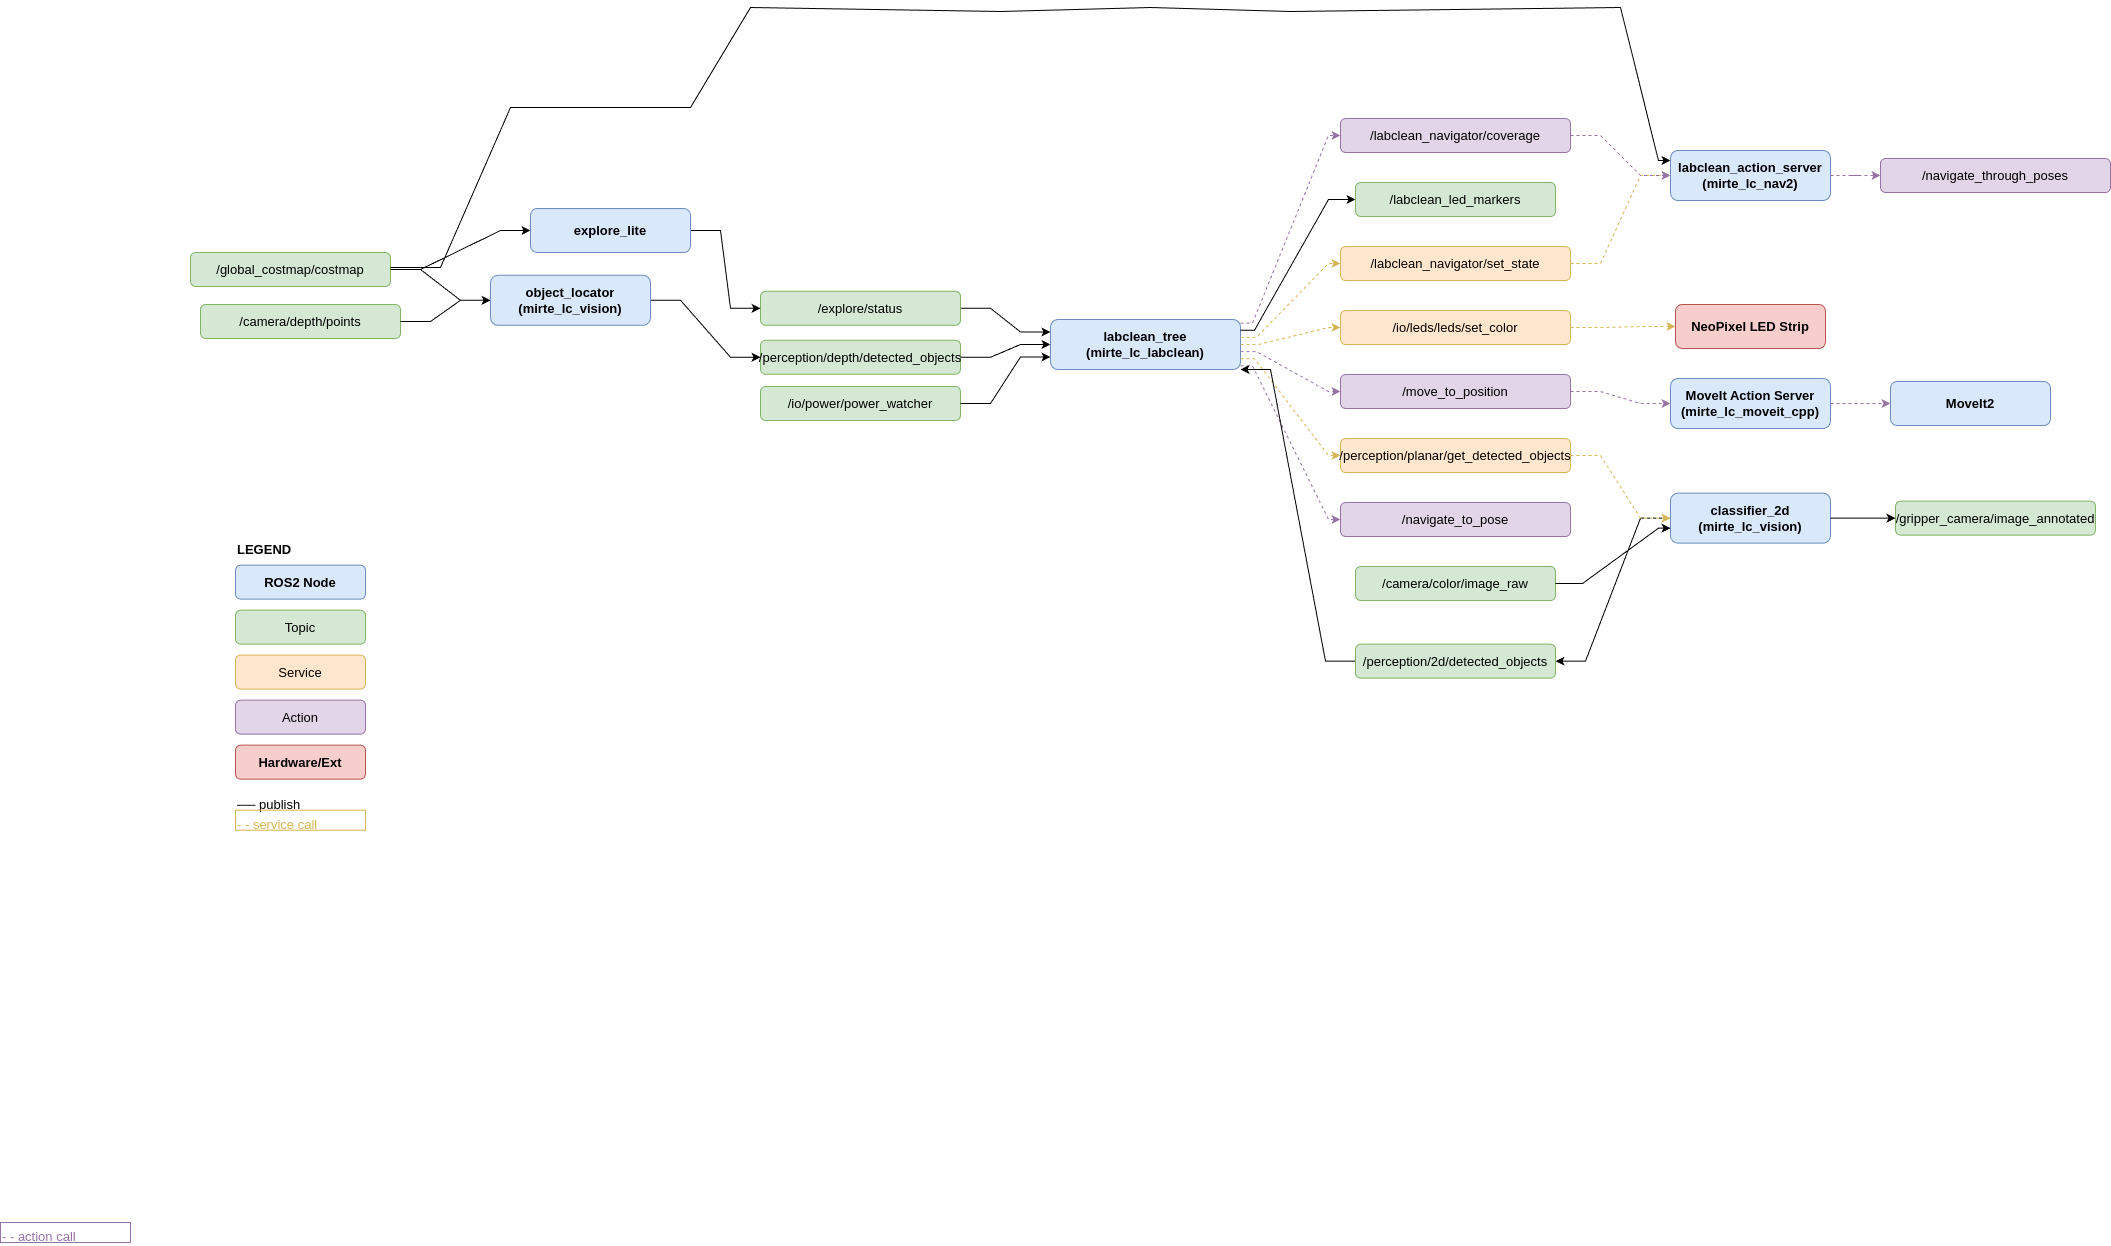
\includegraphics[width=0.82\linewidth]{content/figures/ros2_topic_diagram.png}
    \caption{ROS 2 architecture.}
    \label{fig:arch}
\end{figure}

\begin{paracol}
    {2}
    \subsection{Simulation}
    Development began without access to a physical robot. A Gazebo simulation environment was therefore set up to allow the software stack to be developed and tested in the interim. The simulated environment can be explored interactively in the online version of this report.

    \subsection{Sim-to-Real Pipeline}
    For the transition from simulation towards real-world testing, the codebase needed to be adapted. The launch files were modified so that Gazebo was no longer used and \texttt{use\_sim\_time} parameters were set to \texttt{false}. To reduce the risk of collisions, the inflation radius and the robot radius in the Nav2 parameters were increased. Another change was the migration of processing tasks from the Orange Pi 3B to a laptop connected to the MIRTE. Finally, all the sensors were tested and it was concluded that the depth camera was not positioned correctly, so its position was changed from the front of the robot to the gripper, allowing its viewing angle and distance to the object to be adjusted more effectively.

    \syncallcounters
    \switchcolumn
    \subsection{Testing Environment}
    For testing, an open, medium-sized room was chosen. The room needed to have sufficiently large open spaces for the robot to be able to plan its trajectories for the object-detection phase. Due to the use of mecanum wheels and camera-based object detection, the room also needed to have a mostly smooth, flat floor with a uniform colour.

    \medskip
    \centerline{\rule{7.8cm}{0.4pt}}
    \subsection{Testing Objects}
    Due to the low video output quality of the included USB camera module, including significant motion blur and difficulties with exposure under different lighting conditions, the success rate of recognition and classification of electronic objects was too low. Additionally, most electronic waste had too low a profile to be recognized reliably by the depth camera. As a result, it was decided to 3D-print coloured shapes with a textured outer wall for grip. A custom dataset was created for the object-classification model to improve object-detection performance.
\end{paracol}

\section{Results}
    This section covers the observed characteristics of the implemented coverage planners, perception methods and solutions regarding manipulation. 
    \subsection{Coverage Planners}
    Three path planners have been compared:
    \begin{itemize}
    \item Boustrophedon Coverage
    \item Morphology-based Skeleton Coverage
    \item Spanning Tree Coverage
    \end{itemize}

    The Boustrophedon coverage planner package had compatibility issues with other packages used for navigation, which meant that Boustrophedon did not work on the MIRTE Master.

    The morphology-based skeleton coverage planner performed well in laboratory-like environments but worse in larger open spaces. This planner allowed the robot to maneuver efficiently between objects such as tables and chairs while still being able to get into tight places. 
    
    The morphology-based skeleton coverage planner also resulted in the fewest sharp turns, which, given the simple odometry of the MIRTE Master (wheel encoders only), helped the robot keep track of its position and thus keep the map clean. However, the skeleton planner performed slightly worse in terms of coverage performance. This was due to the lower density of the planned path, which sometimes caused the robot to miss the edges of larger free spaces that needed to be scanned for objects.
    
    \begin{figure}[H]
    \centering
    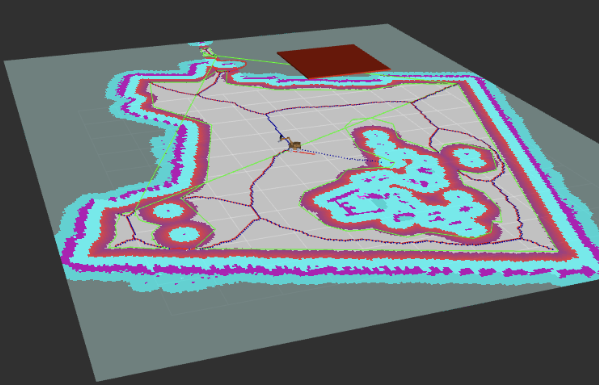
\includegraphics[width=0.99\linewidth]{latex/figures/Screenshot 2026-06-12 at 11.49.17.png}
    \caption{Skeleton path in laboratory environment}
    \label{fig_skeletonpathresult}
    \end{figure}
    
    The spanning tree coverage planner performed well in large open spaces, but unlike the morphology-based skeleton coverage planner, it struggled more with planning paths in tighter spaces such as laboratory environments (see Figure \ref{fig_spanningtreeresults}), resulting in separate path loops being stitched together and, possibly, tighter spots between the loops being missed. Also, because of the nature of the coverage pattern, many small-radius turns are generated, which sometimes caused the robot to slowly accumulate drift in the odometry, resulting in less accurate localization and a less accurate map.
    
    \begin{figure}[H]
    \centering
    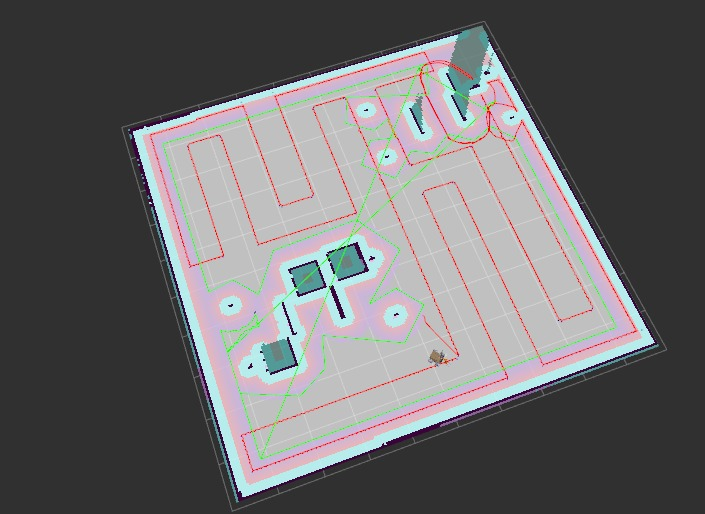
\includegraphics[width=0.99\linewidth]{latex/figures/SpanningTreeResult.jpeg}
    \caption{Spanning tree path in laboratory environment}
    \label{fig_spanningtreeresults}
    \end{figure}
    \subsection{Object Localization and Classification}
     For object detection, a localization method and a classification method were developed. Our object localizer relies on bounding boxes that are retrieved from point clouds generated from the depth camera's depth images. Our object detector was able to find objects sized from 1\,cm to 6\,cm. A bounding box drawn around a found object in the point cloud is shown in Figure \ref{fig_boundingboxesandyolo}. The custom-made YOLO26 object-detection model worked as intended, correctly classifying the localized objects. Figure \ref{fig_boundingboxesandyolo} also shows a frame from the RGB sensor of the depth camera in the bottom-right corner.
        \begin{figure}[H]
    \centering
    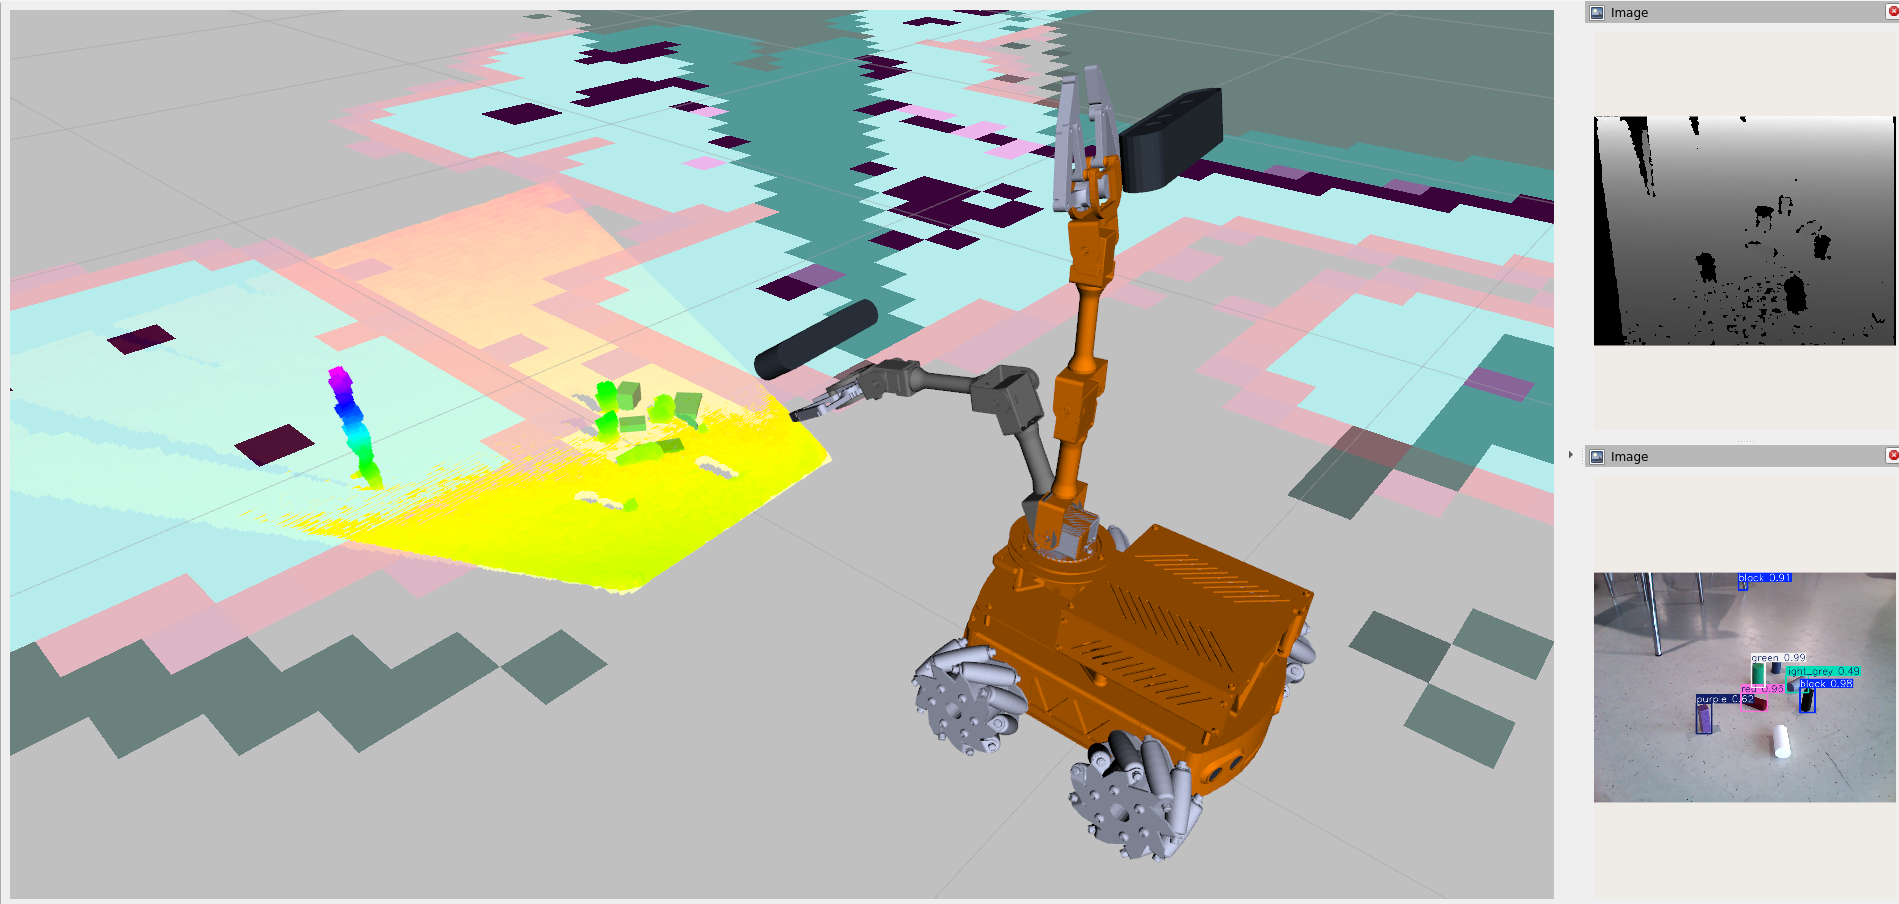
\includegraphics[width=0.9\linewidth]{latex/figures/BoundingBoxYolo.png}
    \caption{Bounding box drawn around found objects (center) and YOLO26 working simultaneously (bottom right)}
    \label{fig_boundingboxesandyolo}
    \end{figure}
    \subsection{Manipulation}
    \paragraph{Movement accuracy}
    The manipulation of the actuator has seen major improvements regarding movement accuracy. The initial accuracy of the actuator was around 15\,cm. After the code was reworked, the actuator was controlled by actual joint values instead of approximations. This reduced the error significantly, resulting in a movement error of only 1\,mm.

    \paragraph{Gripping performance}
    The gripping performance of the original robot was slightly improved by adding rubberized patches to the gripping surfaces of the gripper. This has significantly helped the gripper hold the smooth, plastic testing objects when it approached them at a sub-optimal angle.
    \begin{figure}[H]
    \centering
    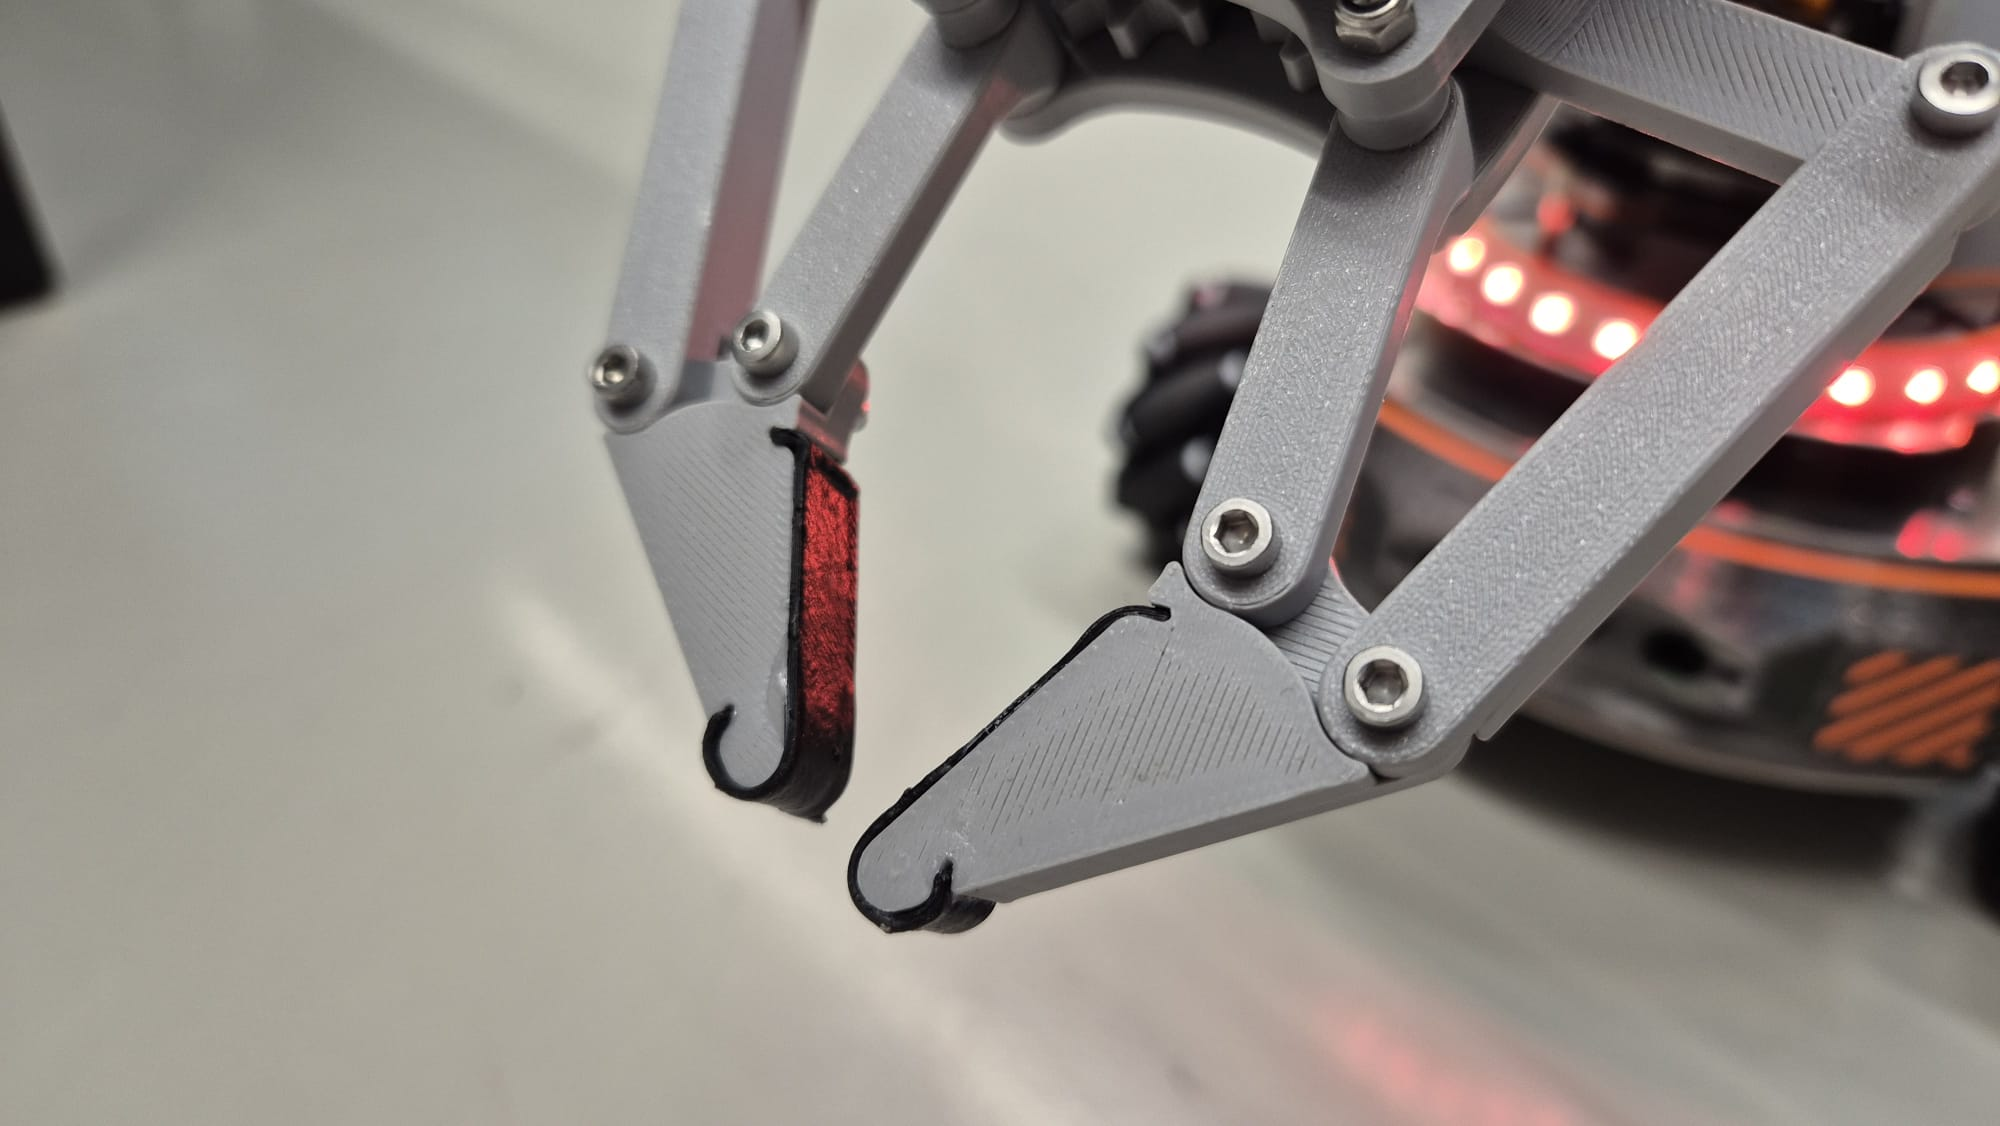
\includegraphics[width=0.99\linewidth]{latex/figures/RubberizedGrippingSurfaces.jpeg}
    \caption{Rubberized gripping surfaces.}
    \label{fig_rubberizedgrippingsurfaces}
    \end{figure}


\section{Discussion}

\subsection{Delays}

We were caught in the middle of a platform migration to a new design. This migration happened at the time that a master's course started, which used up all of the available MIRTE Master robots. This meant that, for us, no robot was available from the start of the project. We also had no clarity about when a unit would be received and whether additional components needed to be ordered, and we could not order all components ourselves because of budget restrictions. In the end, the components were received in week 13 of the 16-week project period. While the software team was able to front-load much of the development using Gazebo simulations, this still meant that the team had only three weeks to discover the quirks of the MIRTE Master, troubleshoot them, and integrate the software, which severely limited our ability to perform real-world quantitative and qualitative experiments.

\subsection{Gazebo}

Gazebo was a useful tool for testing the software stack quickly and in an isolated manner. However, learning to work with Gazebo required a steep learning curve and a significant amount of additional effort to set up a realistic environment, including custom worlds and interactive objects.

When transferring the code base from the simulation environment to the real world, several problems occurred. The code had to be adjusted, for example by avoiding \texttt{use\_sim\_time}, and the robot's sensors were found to provide less accurate and less reliable feedback than expected.

\subsection{The MIRTE Master Platform}

The MIRTE Master proved to be a viable starting platform for a cleaning robot. Much of the required setup was already in place: MoveIt was available, Nav2 for MIRTE was present, Gazebo already existed, and many of the configuration files and calibrations were operational.

However, some parts of the design were not tested as thoroughly as expected before integration into the MIRTE Master platform. The most significant issues were found in the perception components. The RGB-D camera was initially mounted near the front and lower part of the robot, which resulted in depth images that were not suitable for point-cloud processing. The included USB camera module was also excluded from the final design because of poor performance, including motion blur and a pronounced drop in frame rate under changing lighting conditions.

The final major issue encountered was time synchronization between the MIRTE Master and other machines. The Orange Pi 3B on the MIRTE Master was not powerful enough to run the full software stack on its own, so much of the processing had to be offloaded to a laptop. For this to work correctly, the time needed to be synchronized between the devices. Later, a custom implementation based on \href{https://chrony-project.org/}{Chrony} was used to synchronize the clocks automatically within acceptable tolerances.

In addition, the implemented navigation and perception approaches were feasible but not yet fully optimized. The coverage planners traded off completeness against path smoothness, and the perception pipeline remained sensitive to lighting and object appearance. These limitations provide useful guidance for future work.

\section{Conclusion}

This work has demonstrated that the different coverage planners each have distinct strengths and weaknesses. The morphology-based skeleton planner performed well in cluttered environments with tight spaces, while the spanning-tree planner provided better coverage in larger open spaces at the cost of more sharp turns and less accurate localization.

The developed perception pipeline successfully localized and classified small objects, demonstrating that this combination is an effective solution for object recognition on the MIRTE Master. The modifications to the manipulator also substantially improved positioning accuracy and grasp reliability, making objects manipulable even at less favorable approach angles.

Overall, this work has shown that the MIRTE Master can accommodate the components required for a laboratory-cleaning robot and is therefore a viable platform for this task. At the same time, the results also show that further improvements in sensing hardware, perception robustness, and testing procedures would be necessary before the system could be deployed more widely.

\subsection{Future Work}

Future research can use the software packages created as part of this work to evaluate the performance of the robot by testing the different coverage planners in isolation and in combination with the rest of the system. Additionally, other coverage planners, such as Voronoi-based \cite{voronoi} and boustrophedon \cite{Choset1997} planners, can be implemented and tested. It could also be interesting to observe the influence of different environments on the overall performance of the system. Another possible avenue for future research is porting the MIRTE Master software stack to a more suitable single-board computer and observing differences in computational performance.

\end{multicols}

%\include{latex/latex_export/report_tex-discussion}

% --- Disabled: stale MyST export (old text, gray). It cannot be \include'd when compiling from latex/
% --- (its .aux files need latex/latex/latex_export) and it references figures that are not in the repo.
% --- Re-run the 'MyST PDF builder [LaTeX]' workflow and re-enable if you want to compare against it.
% \color{gray}
%
% \include{latex/latex_export/report_tex-introduction}
% %\include{latex/latex_export/report_tex-theory}
% \include{latex/latex_export/report_tex-systemoverview}
% \include{latex/latex_export/report_tex-mechanical}
% \include{latex/latex_export/report_tex-navigation}
% \include{latex/latex_export/report_tex-coverageplanners}
% \include{latex/latex_export/report_tex-perception}
% \include{latex/latex_export/report_tex-perception2d}
% \include{latex/latex_export/report_tex-perception3d}
% \include{latex/latex_export/report_tex-methods}
% \include{latex/latex_export/report_tex-results}
% \include{latex/latex_export/report_tex-conclusion}
% \include{latex/latex_export/report_tex-materials}
%
% \color{black}

\clearpage % appendix starts on a new page
\section{Appendix}
\subsection{Algorithms}
% ┌─────────────────────────────────────────────────────────────┐
% │ SECTION 1 — Coverage Path Planning (SkeletonPlanner)        │
% └─────────────────────────────────────────────────────────────┘

\begin{algorithm}
\footnotesize
\caption{Skeleton-Based Coverage Path Planning}
\label{alg:skeleton}
\KwIn{Occupancy grid $\mathcal{M}$, robot start position $\mathbf{p}_0 \in \mathbb{R}^2$}
\KwOut{Ordered list of waypoint segments $\mathcal{P} = [P_1, P_2, \ldots, P_k]$}

\tcc{Map preprocessing}
$B \leftarrow$ threshold($\mathcal{M}$, lethal\_threshold) \tcp*{binary free-space mask}
$C \leftarrow$ extractContours($B$) \tcp*{OpenCV RETR\_TREE}
$G_{poly} \leftarrow$ groupContoursByContainment($C$) \tcp*{outer + holes}

\ForEach{polygon group $g \in G_{poly}$}{
    $S \leftarrow$ medialAxis($B$) \tcp*{skimage skeletonize}
    $W \leftarrow$ skeletonToWorldCoords($S$)\;
    $G_{graph} \leftarrow$ buildKDTreeGraph($W$, radius $= r_{path}$)\;
    bridgeDisconnectedComponents($G_{graph}$)\;

    $L \leftarrow$ findLeafNodes($G_{graph}$) \tcp*{nodes with degree 1}
    $v \leftarrow$ nearestLeaf($\mathbf{p}_0$, $L$)\;
    $\mathcal{Q} \leftarrow [v]$, $\;V_{visited} \leftarrow \emptyset$\;

    \While{$V_{visited} \neq L$}{
        $V_{visited} \leftarrow V_{visited} \cup \{v\}$\;
        $r \leftarrow$ nearestLeafByGraphDistance($v$, $L \setminus V_{visited}$, $G_{graph}$)\;
        $\pi \leftarrow$ shortestPath($v$, $r$, $G_{graph}$) \tcp*{Dijkstra}
        append $\pi$ to $\mathcal{Q}$\;
        $v \leftarrow r$\;
    }

    $P_i \leftarrow [W[u]\;\forall\,u \in \mathcal{Q}]$\;
    append $P_i$ to $\mathcal{P}$\;
    $\mathbf{p}_0 \leftarrow P_i[\text{last}]$ \tcp*{chain segments}
}
sanitiseWaypoints($\mathcal{P}$, $\mathcal{M}$) \tcp*{clamp to costmap bounds}
\Return $\mathcal{P}$
\end{algorithm}

% ┌─────────────────────────────────────────────────────────────┐
% │ SECTION 6 — Spanning Tree Coverage Path Planning            │
% └─────────────────────────────────────────────────────────────┘


\begin{algorithm}[H]
\footnotesize
    \caption{Spanning-Tree Coverage Path Planning}
    \label{alg:spanning_tree}
    \KwIn{Occupancy grid $\mathcal{M}$, robot start position $\mathbf{p}_0 \in \mathbb{R}^2$, scale factor $s = 0.06$}
    \KwOut{Ordered list of waypoint segments $\mathcal{P} = [P_1, P_2, \ldots, P_k]$}
    
    \tcc{Map preprocessing}
    $B \leftarrow$ threshold($\mathcal{M}$, lethal\_threshold) \tcp*{binary free-space mask}
    $B_{down} \leftarrow$ resize($B$, scale $= s$, interpolation $=$ NEAREST) \tcp*{downsample}
    
    \tcc{Build spanning tree over free cells}
    $G \leftarrow$ gridGraph($B_{down}$) \tcp*{4-connected grid graph}
    \ForEach{edge $(u, v) \in G$}{
        \If{$B_{down}[u] = 0$ \textbf{or} $B_{down}[v] = 0$}{
            remove $(u, v)$ from $G$\;
        }
    }
    $T \leftarrow \emptyset$\;
    \ForEach{connected component $\mathcal{C} \in G$}{
        $T \leftarrow T \cup$ DFS\_tree($\mathcal{C}$)\;
    }
    
    \tcc{Edge subdivision — insert midpoint nodes}
    \ForEach{edge $(u, v) \in T$}{
        $m \leftarrow \frac{u + v}{2}$\;
        replace $(u,v)$ with $(u,m)$ and $(m,v)$\;
    }
    
    \tcc{Generate circumnavigation contours}
    $P_{perim} \leftarrow \mathbf{0}^{H \times W}$ \tcp*{blank perimeter map}
    $r \leftarrow \lfloor \frac{1}{4s} \rfloor$ \tcp*{rectangle half-size in pixels}
    \ForEach{node $p \in T$}{
        $p_{img} \leftarrow \frac{p + 0.5}{s}$ \tcp*{scale back to image coords}
        drawFilledRect($P_{perim}$, centre $= p_{img}$, halfsize $= r$)\;
    }
    $\mathcal{C} \leftarrow$ findContours($P_{perim}$, RETR\_EXTERNAL)\;
    
    \tcc{Convert contours to world-frame waypoints and plan}
    $\mathcal{P} \leftarrow [\;]$\;
    \ForEach{contour $c \in \mathcal{C}$}{
        $W \leftarrow$ pixelToWorld($c$)\;
        \If{$|W| < 2$}{\textbf{continue}\;}
        $idx \leftarrow \arg\min_{i} \| W[i] - \mathbf{p}_0 \|_2$ \tcp*{start from nearest point}
        $P_i \leftarrow [W[idx], W[idx+1], \ldots, W[-1], W[0], \ldots, W[idx-1]]$\;
        append $P_i$ to $\mathcal{P}$\;
        $\mathbf{p}_0 \leftarrow P_i[\text{last}]$\;
    }
    sanitiseWaypoints($\mathcal{P}$, $\mathcal{M}$)\;
    \Return $\mathcal{P}$
\end{algorithm}

% ┌─────────────────────────────────────────────────────────────┐
% │ SECTION 2 — Coverage Execution with Pause/Resume            │
% └─────────────────────────────────────────────────────────────┘

\begin{algorithm}
\small
\caption{Coverage Task Execution with Pause/Resume}
\label{alg:coverage_exec}
\KwIn{Coverage segments $\mathcal{P}$, planner type $\tau$}
\KwOut{Task result (success / cancelled / stopped)}

$\mathcal{P} \leftarrow$ sortByLength($\mathcal{P}$, descending)\;
$n \leftarrow |\mathcal{P}|$, $\;i \leftarrow 0$\;

\While{$\mathcal{P} \neq \emptyset$}{
    $P_i \leftarrow$ dequeue($\mathcal{P}$), $\;i \leftarrow i + 1$\;
    nav2.goThroughPoses(toROSPath($P_i$))\;

    \Repeat{nav2.isTaskComplete()}{
        $f \leftarrow$ nav2.getFeedback()\;
        publishFeedback($i$, $n$, $f$.remainingPoses)\;

        \If{cancelRequested}{
            nav2.cancelTask()\;
            \Return CANCELLED\;
        }
        \If{stopRequested}{
            nav2.cancelTask()\;
            \Return STOPPED\;
        }
        \If{pauseRequested}{
            nav2.cancelTask()\;
            $P_{rem} \leftarrow$ computeRemainingSegment($P_i$, getRobotPos())\;
            prepend $P_{rem}$ to $\mathcal{P}$ \tcp*{resume from current pose}
            \Repeat{\textbf{not} pauseRequested}{spinOnce()}\;
            nav2.goThroughPoses(toROSPath($P_{rem}$))\;
        }
    }
    publishFeedback($i$, $n$, 0)\;
}
\Return SUCCESS
\end{algorithm}


% ┌─────────────────────────────────────────────────────────────┐
% │ SECTION 3 — 3D Object Detection Pipeline                    │
% └─────────────────────────────────────────────────────────────┘

\begin{algorithm}
\caption{Depth-Based Object Detection}
\label{alg:object_detection}
\KwIn{Point cloud $\mathcal{C}$ (camera frame), costmap $\mathcal{M}$, TF tree}
\KwOut{Detected object array $\mathcal{O}$}

$\mathcal{C} \leftarrow$ removeNaN($\mathcal{C}$)\;
$\mathcal{C}_{LQ} \leftarrow \mathcal{C}$, $\;mask \leftarrow \mathbf{1}^{|\mathcal{C}|}$\;

\tcc{Iterative RANSAC plane removal}
\Repeat{$|\mathcal{C}_{LQ}| < 100$ \textbf{or} $|\text{inliers}| < 500$}{
    $(\mathbf{n}, d) \leftarrow$ RANSAC\_segmentPlane($\mathcal{C}_{LQ}$,\;
    $\quad\epsilon=0.003$,\; $n_{iter}=2000$)\;
    $\mathcal{C}_{LQ} \leftarrow \mathcal{C}_{LQ} \setminus$ inliers\;
    $mask \leftarrow mask \;\wedge\; (\text{dist}(\mathcal{C}, \Pi) > 0.008)$\;
}
$\mathcal{C}_{obj} \leftarrow \mathcal{C}[mask]$\;
\tcc{Coordinate transform to map frame}
$T_{cam \to base} \leftarrow$ TF.lookup(base\_link, camera\_frame)\;
$T_{base \to map} \leftarrow$ TF.lookup(map, base\_link)\;
$\mathcal{C}_{map} \leftarrow T_{base \to map} \cdot T_{cam \to base} \cdot \mathcal{C}_{obj}$\;

\tcc{Costmap filtering}
$\mathcal{C}_{map} \leftarrow \{\mathbf{p} \in \mathcal{C}_{map} : \mathcal{M}(\mathbf{p}) < \delta_{occ}\}$\;

\tcc{Clustering and bounding box extraction}
$L \leftarrow$ DBSCAN($\mathcal{C}_{map}$, $\varepsilon=0.03$, minPts$=20$)\;
$\mathcal{O} \leftarrow [\;]$\;
\ForEach{cluster $k \in L,\; k \neq -1$}{
    $OBB_k \leftarrow$ getOrientedBoundingBox($\mathcal{C}_{map}[L{=}k]$)\;
    \If{$\mathcal{M}(OBB_k.\text{center}) < \delta_{occ}$}{
        $\psi \leftarrow$ arctan2($R_k[1,0]$, $R_k[0,0]$) \tcp*{yaw only}
        append DetectedObject($OBB_k$.center, $OBB_k$.extent, $\psi$) to $\mathcal{O}$\;
    }
}
\Return $\mathcal{O}$
\end{algorithm}

\clearpage % each appendix part starts on a new page (also flushes the algorithm floats)
\begin{multicols}{2}
\subsection{Materials}
    %Within this section, all hardware employed within the MIRTE Master will be displayed and discussed.

    \subsubsection{Hardware Specifications}

    Most of the hardware used in this implementation of the MIRTE Master comes from the standard components provided by the MIRTE team. The list of hardware parts, which excludes only trivial components such as nuts and bolts, can be found on the \href{https://matt-rbt.github.io/Lab-Cleanup-Robot-using-the-Mirte-Master-Platform/materials/}{Materials} web page. Given that MIRTE is not produced in large quantities and no standardized spare parts are available, 3D-printing was a practical way to produce the required structural parts from adjusted versions of the provided CAD models. These parts can be divided into two groups: chassis and manipulator.
    

    \subsubsection{Chassis}
    
    The chassis consists of a top, bottom, and manipulator-mounting plate, for which aluminium plates with a thickness of 1.5 mm were used, as well as several side panels. These side panels not only act as chassis support elements but also serve as mounting points for several electronic components. For these purposes, PETG was chosen because it is easy to print, impact-resistant, and sufficiently stiff for the intended application. The aluminium plates were chosen for their rigidity and durability. Although no formal material tests were performed in this study, these choices were made to match the practical requirements of the robot's payload and expected handling. \newline
    
    The translucent PETG variant used for this project also enables the user to look at the status lights on the inside of the chassis. This would otherwise not have been possible due to the aluminium top and bottom plates. During printing, orange PETG accent lines were also added to make the robot more visible to people passing by.
    \subsubsection{Manipulator}
    
    The manipulator consists of several components, which are listed on the \href{https://matt-rbt.github.io/Lab-Cleanup-Robot-using-the-Mirte-Master-Platform/materials/}{Materials} web page. This system can be divided into four groups: brackets, limbs, servo-motors, and the gripping mechanism. Given that there are four servo-motors, the arm is defined to have four degrees of freedom to be able to reach all places around the robot.

    There is a fifth servo-motor mounted, but it only actuates the gripping mechanism and therefore does not add any degree of freedom to the system. All of this, including the chassis, can be seen in the interactive display near the bottom of the \href{https://matt-rbt.github.io/Lab-Cleanup-Robot-using-the-Mirte-Master-Platform/mechanical}{Mechanical} overview page.
    
    \subsubsection{Software specifications}

    The MIRTE Master robotic platform has free open-source software available for any user to install. \newline
    The latest stable release is used in this robotic system. This software comes packaged inside a ROS application \cite{ROS2_2022}, a standardized framework for developing distributed robotic systems. This allows for the use of a wide variety of cross-compatible plugins and additional software packages, making rapid prototyping and development more efficient.
    
    The ROS distribution used by the MIRTE Master platform is ROS 2 Humble Hawksbill on Ubuntu 22.04.
    

    \paragraph{SLAM}
    Before the robot is able to perform any complex task in an environment, the environment must first be mapped. For this, SLAM (Simultaneous Localization and Mapping) is used. This way, the robot can dynamically update its map of the environment based on measurements from its LiDAR scanner.
    The robot creates an occupancy grid map, represented as an image, while estimating its own pose.
    The two most widely adopted SLAM frameworks in the ROS ecosystem are Cartographer \cite{cartographer} and SLAM Toolbox \cite{SlamTBX2021}. For the MIRTE Master platform, SLAM Toolbox was selected due to its superior mapping accuracy and localization performance when reliable odometry is available \cite{slamvscart}. Since the MIRTE Master is dedicated to running the core robotics software stack and is not burdened by other computationally intensive workloads, the higher computational requirements of SLAM Toolbox do not pose a significant limitation. Consequently, prioritizing mapping accuracy over computational efficiency makes SLAM Toolbox the most suitable choice for this application.
    SLAM Toolbox was also chosen for its native ROS 2 support and good integration with other ROS 2 packages. SLAM Toolbox allows for straightforward modification of mapping behavior using the set of parameters it provides. In the case of the MIRTE Master, there are several projects that have implemented SLAM Toolbox, so finding a ready-to-use set of SLAM parameters for this robot is relatively simple. The \href{https://github.com/MartijnWisse/mirte\_navigation}{Mirte Navigation} ROS package is used as a starting point for configuration files and SLAM parameter settings.
    It was assumed that the robot would only navigate in unknown environments without predefined or recurring maps. Localization (using AMCL) was therefore disabled in the application.
    \paragraph{Manipulation}

    While the arm on the MIRTE Master can be controlled in joint-space, the implementation relies on task-space (Cartesian-space) control over the end-effector position. \newline
    The manner in which motion planners are typically implemented requires the integration of several complex subsystems, such as inverse and forward kinematics solvers, trajectory planners, and path planners. To accomplish the goal of task-space control over the arm, MoveIt 2 (\cite{Coleman2014MoveIt}) was used.
    
    
    \paragraph{Navigation}
    Robot navigation poses a challenge analogous to that of robot manipulation: workspace control. The robot must be able to navigate to or through a set of waypoints given in the coordinate system of the map, while also implementing a real-time controller for obstacle avoidance. Similar to MoveIt 2, Nav2 is used as a solution to this problem (\cite{macenski2020marathon2}). Aside from path planning and real-time control, Nav2 also provides a \href{https://docs.nav2.org/configuration/packages/configuring-costmaps.html}{Costmap}.


\end{multicols}

\clearpage
\subsection{Figures}
    \begin{figure}[H]
        \centering
        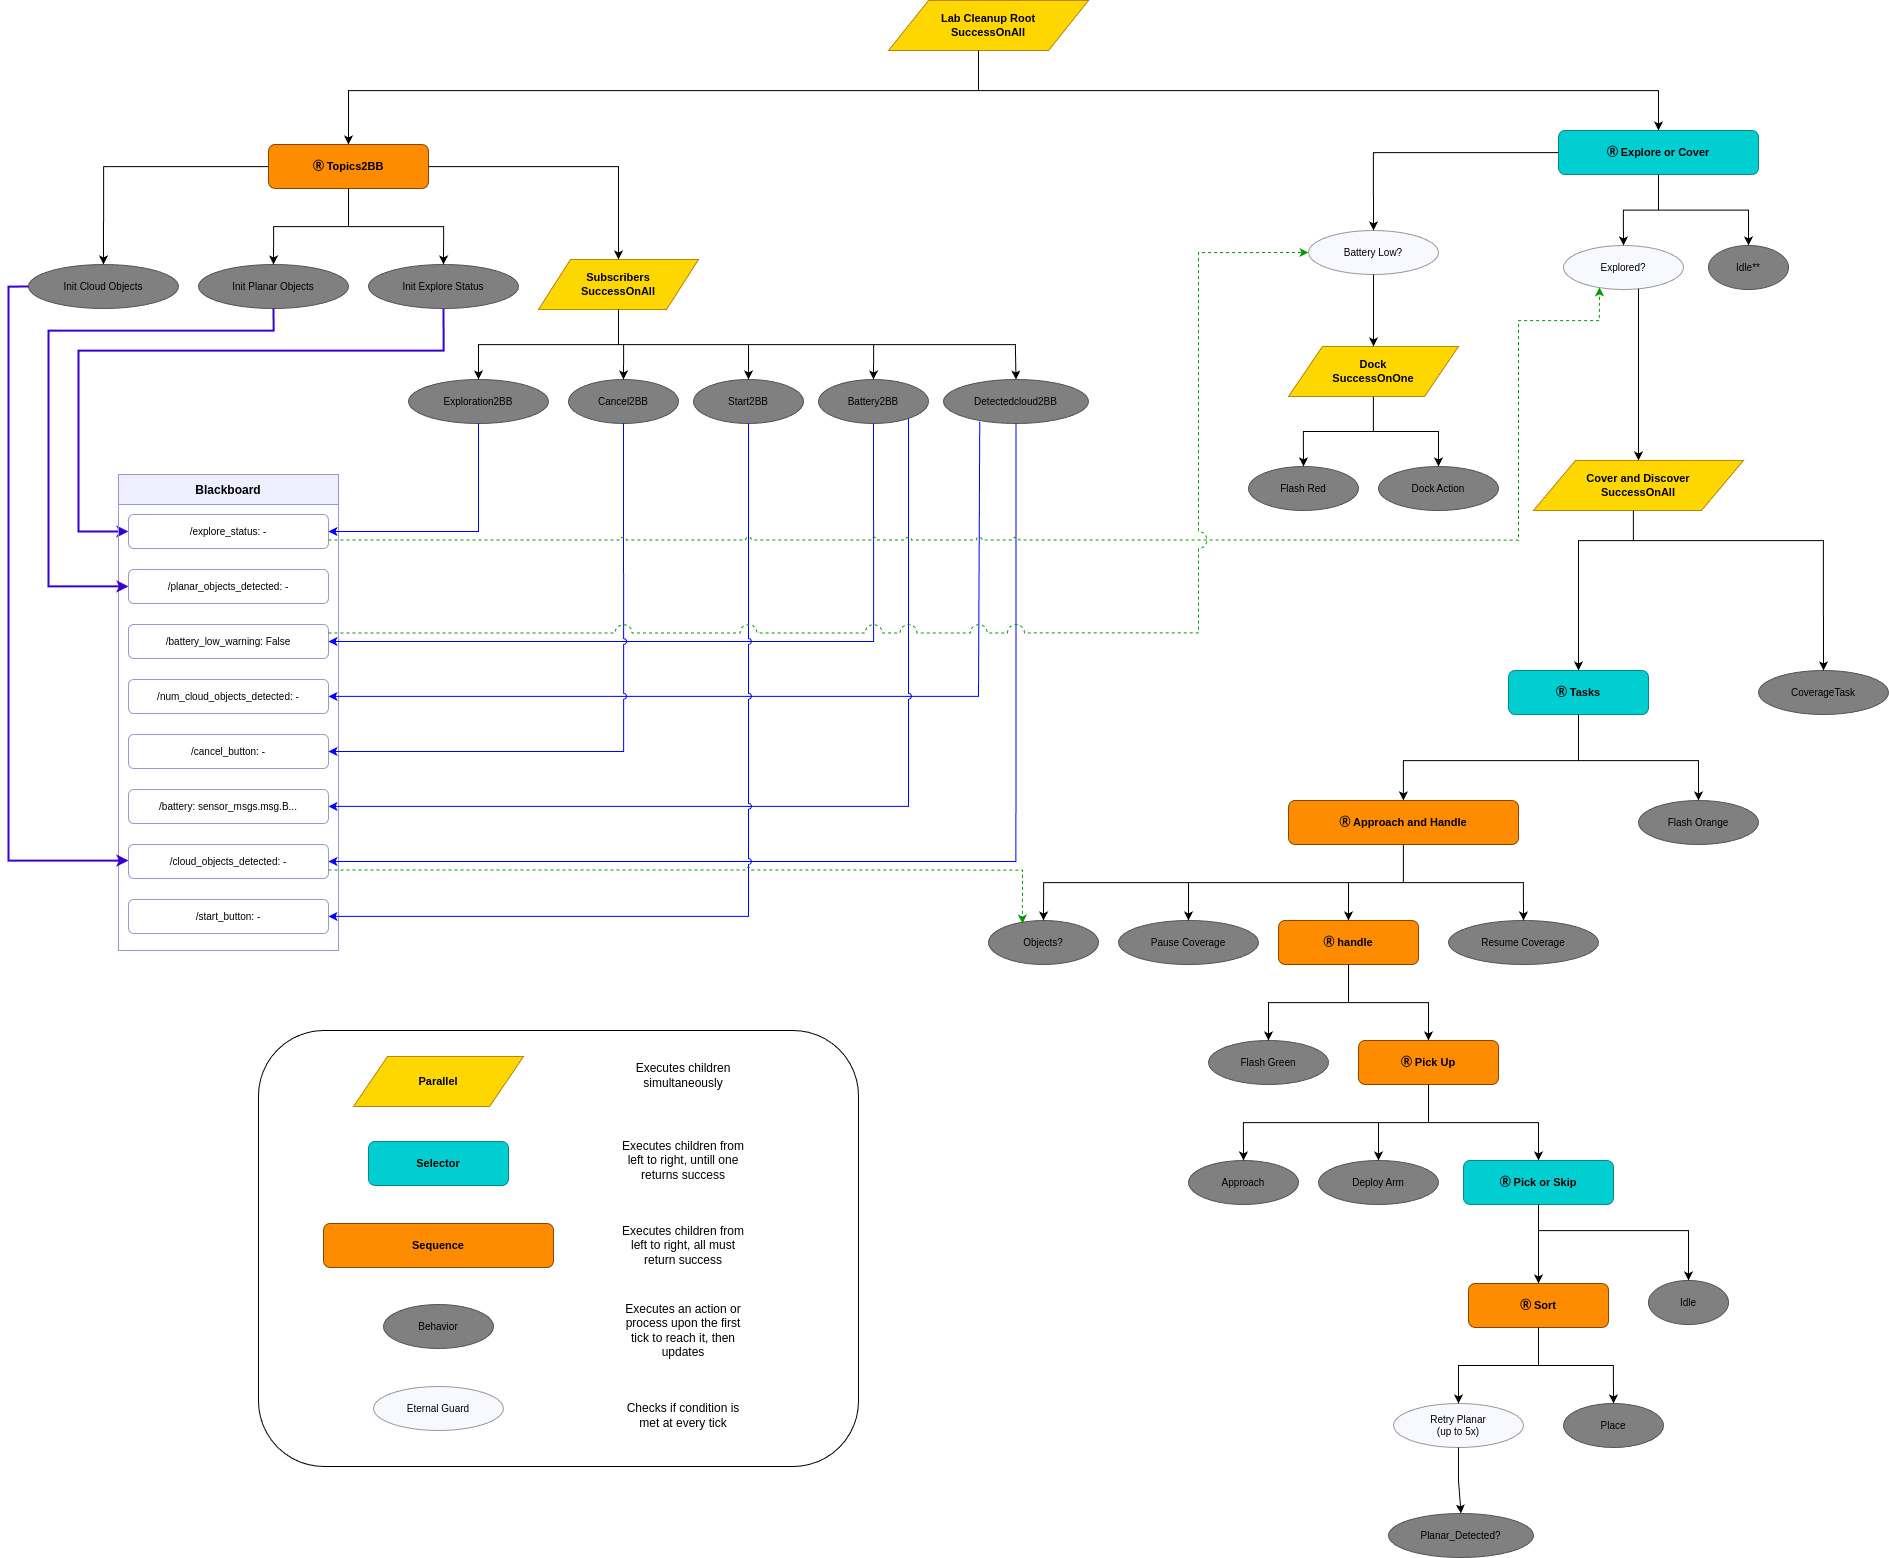
\includegraphics[width=0.99\linewidth]{latex/figures/labcleantree.png}
        \caption{Full Behavior Tree}
        \label{fig:tree_full}
    \end{figure}

%%%%%%%%%%%%%%%%%%%%%%%%%%%%%%%%%%%%%%%%%%%%%%%%%%
%%%%%%%%%%%%%%  acronyms & glossary  %%%%%%%%%%%%%
\printglossaries
%%%%%%%%%%%%%%%%%%%%%%%%%%%%%%%%%%%%%%%%%%%%%%%%%%

\clearpage
%% \bibliographystyle{IEEEtranN}
% \bibliography{main}
\printbibliography[heading=bibintoc,title={References}]
\end{document}